% ****** Start of file apssamp.tex ******
%
%   This file is part of the APS files in the REVTeX 4.1 distribution.
%   Version 4.1r of REVTeX, August 2010
%
%   Copyright (c) 2009, 2010 The American Physical Society.
%
%   See the REVTeX 4 README file for restrictions and more information.
%
% TeX'ing this file requires that you have AMS-LaTeX 2.0 installed
% as well as the rest of the prerequisites for REVTeX 4.1
%
% See the REVTeX 4 README file
% It also requires running BibTeX. The commands are as follows:
%
%  1)  latex apssamp.tex
%  2)  bibtex apssamp
%  3)  latex apssamp.tex
%  4)  latex apssamp.tex
%
\documentclass[%
reprint,
 superscriptaddress,
%groupedaddress,
%unsortedaddress,
%runinaddress,
%frontmatterverbose, 
%  preprint,
%showpacs,preprintnumbers,
%nofootinbib,
%nobibnotes,
%bibnotes,
 amsmath,amssymb,
 aps,
%pra,
%prb,
%rmp,
%prstab,
%prstper,
%floatfix,
]{revtex4-1}

\usepackage{graphicx}% Include figure files
\usepackage{dcolumn}% Align table columns on decimal point
\usepackage{bm}% bold math
\usepackage{color}
%\usepackage{hyperref}% add hypertext capabilities
%\usepackage[mathlines]{lineno}% Enable numbering of text and display math
%\linenumbers\relax % Commence numbering lines

%\usepackage[showframe,%Uncomment any one of the following lines to test 
%%scale=0.7, marginratio={1:1, 2:3}, ignoreall,% default settings
%%text={7in,10in},centering,
%%margin=1.5in,
%%total={6.5in,8.75in}, top=1.2in, left=0.9in, includefoot,
%%height=10in,a5paper,hmargin={3cm,0.8in},
%]{geometry}
\usepackage{makecell}
\usepackage{listings}
\usepackage{xspace}

\lstset{basicstyle=\ttfamily}
% \lstset{showstringspaces=false}
\lstset{columns=fullflexible}
% \lstset{keepspaces=true}
\lstset{frame=single}
\lstset{numbers=right}

\newcommand\nd{\textsuperscript{nd}\xspace}
\newcommand\rd{\textsuperscript{rd}\xspace}
\newcommand\nth{\textsuperscript{th}\xspace} %\th is taken already

\def\V{\mathcal{V}}
\def\C{\mathcal{C}}
\def\P{\mathcal{P}}
\def\NMC{{N_{\mathrm{MC}}}}
\def\NpMC{{N'_{\mathrm{MC}}}}
\def\NppMC{{N''_{\mathrm{MC}}}}
\def\NMCdiff{{N_{\mathrm{MC}}^{\mathrm{diff}}}}
\def\Nd{{N_d}}
\def\Nddiff{{N_{d}^{\mathrm{diff}}}}

\def\beq{\begin{eqnarray}}
\def\eeq{\end{eqnarray}}

\begin{document}

%\preprint{APS/123-QED}

%\title{Homogeneous Electron Gas Simulation with\\
%Fast Semistochastic Heat-Bath Selected Configuration Interaction}% Force line breaks with \\
%\thanks{J.L. and C.J.U acknowledge support from the National Science Foundation under grant ACI-1534965.}
\title{Correlation Energy of the Homogeneous Electron Gas Simulation from the\\
Semistochastic Heatbath Configuration Interaction Method}% Force line breaks with \\

\author{Junhao Li}
  \email{jl2922@cornell.edu}
  \affiliation{Laboratory of Atomic and Solid State Physics, Cornell University, Ithaca, New York 14853, United States}
\author{Adam Holmes}
  \affiliation{Laboratory of Atomic and Solid State Physics, Cornell University, Ithaca, New York 14853, United States}
\author{Frank Petruzielo}
 %\altaffiliation[Also at ]{Physics Department, XYZ University.}%Lines break automatically or can be forced with \\
\author{C. J. Umrigar}%
  \email{CyrusUmrigar@cornell.edu}
 %\email{Second.Author@institution.edu}
  \affiliation{Laboratory of Atomic and Solid State Physics, Cornell University, Ithaca, New York 14853, United States}

%\collaboration{MUSO Collaboration}%\noaffiliation

%\author{Charlie Author}
% \homepage{http://www.Second.institution.edu/~Charlie.Author}
%\affiliation{
% Second institution and/or address\\
% This line break forced% with \\
%}%
%\affiliation{
% Third institution, the second for Charlie Author
%}%
%\author{Delta Author}
%\affiliation{%
% Authors' institution and/or address\\
% This line break forced with \textbackslash\textbackslash
%}%

%\collaboration{CLEO Collaboration}%\noaffiliation

\date{\today}% It is always \today, today,
             %  but any date may be explicitly specified
%\begin{abstract}
We apply the recently developed fast semistochastic heat-bath configuration interaction (SHCI) to homogeneous electron gas (HEG) system in the mid-to-high density regime.
In this regime, the basis-set incompleteness error is the dominating error for second quantization based methods and SHCI works well with large basis sets.
To obtain highly accurate results, we use up to 39,886 orbitals, which are more than an order of magnitude more than previous state-of-the-art calculations with essentially exact methods.
This reduces the basis set incompleteness error significantly and gives much more accurate and reliable extrapolated results for complete basis sets.
We calculate HEG correlation energies for both the 14-electron and 54-electron supercell cases with effective radius $r_s$ ranging from 0.5 to 5.0 and compare our results with previous methods.
\end{abstract}
\begin{abstract}
We apply the recently developed semistochastic heatbath configuration interaction (SHCI) method to the homogeneous electron gas (HEG) in the mid-to-high density regime.
In this regime, the basis-set incompleteness error is the dominant error for
%second quantization based
basis set
methods
%and SHCI works well with large basis sets.
so we extend the SHCI method to handle large basis sets.
To obtain highly accurate results, we use up to 39,886 orbitals, which is more than an order of magnitude larger than
% previous state-of-the-art calculations with essentially exact methods.
the number used in previous state-of-the-art calculations using methods that yield essentially exact results
within a basis set.
%This reduces the basis set incompleteness error significantly and gives much more accurate and reliable extrapolated results for complete basis sets.
This enables accurate extrapolation to the complete basis set limit.
%We calculate HEG correlation energies for both the 14-electron and 54-electron supercell cases with Wigner-Seitz radius $r_s$ ranging from 0.5 to 5.0 and compare our results with previous methods.
We calculate HEG correlation energies for the 14-electron supercell with Wigner-Seitz radius $r_s$ ranging from 0.5 to 5.0,
and for the 54-electron supercell with $r_s=0.5$ and compare our results with earlier calculations.
\end{abstract}
%\pacs{Valid PACS appear here}% PACS, the Physics and Astronomy
                             % Classification Scheme.
%\keywords{Suggested keywords}%Use showkeys class option if keyword
                              %display desired
\maketitle

%\tableofcontents
%\section{Introduction}
The homogeneous electron gas (HEG) is one of the most fundamental models in condensed-matter physics.
With a tunable parameter, the Wigner-Seitz radius $r_s$, controlling the density of the electrons, HEG provides us a simple paradigm for studying interacting fermions problems of a wide range of systems from weakly correlated to strongly correlated.
In addition, HEG is a cornerstone of the density functional theory (DFT).
In the local density approximation (LDA), the local exchange-correlation energy $\epsilon_{xc}$ comes from HEG~\cite{perdew1986density, dahl2013local}. 
And in the parametrization of more accurate exchange-correlation functionals, HEG energies are also used extensively~\cite{lundqvist2013theory}.

The first accurate calculation of HEG ground state energies over a range of $r_s$ using \textit{ab initio} methods comes from the diffusion Monte Carlo (DMC)~\cite{ceperley1980ground}. However, due to the fixed-node approximation, the energies from DMC are not exact and depend heavily on the quality of the trail wavefunctions.
Several attempts have successfully reduced the fixed-node error, but the question of the magnitude of the remaining errors and the new errors introduced by them has never been completely answered~\cite{kwon1998effects, rios2006inhomogeneous}.

The full configuration interaction quantum Monte Carlo (FCIQMC) is another quantum Monte Carlo based method in the second quantized space. It stochastically samples the configuration space to approximate the full configuration interaction (FCI) energy at a reduced computational cost, and achieved a significantly and variationally lower energy for HEG $r_s=0.5$ than DMC~\cite{shepherd2012investigation}.
However, FCIQMC has the basis set incompleteness error and requires a complete basis set (CBS) extrapolation, which in turn introduces an extrapolation error.
In the mid-to-high density regime, the basis set incompleteness error dominates the total errors.
For example, for HEG with $r_s=0.5$ and 14 electrons in each periodic box, the two largest FCIQMC calculations, which use 778 and 1850 orbitals and give $-0.5893(3)$~Ha and $-0.5936(3)$~Ha respectively, a $4.3$~mHa difference, which is much larger than the uncertainty of FCIQMC itself.
Also, FCIQMC uses initiator approximation to skip side the Fermion-sign problem, which introduces the initiator error.
This error can only be reduced by using a large number of walkers, thus also limits the accuracy.

The coupled cluster Monte Carlo (CCMC) method with high excitation levels reproduces the results from FCIQMC for 14 electrons.
It also shows that for HEG in the mid-to-high density regime, excitation levels all the way to four, i.e., CCSDTQ, are necessary to achieve comparable results as FCIQMC~\cite{neufeld2017study}.
However, due to the high computational cost, CCSDTQ with CCMC has only been applied to 14 electrons and 358 orbitals.

The method that we use in this paper is a modified version of the recently proposed fast heat-bath configuration interaction (SHCI).
HCI is a selected configuration interaction plus perturbation method (SCI+PT) and distinguishes from other SCI+PT methods in that it uses precomputed double excitation lists to significantly improve the efficiency in both the variational stage and perturbation stage~\cite{holmes2016heat}.
HCI in its original form requires a large amount of memory in the perturbation stage.
The semistochastic heat-bath configuration interaction (SHCI) eliminates this memory bottleneck by performing stochastic perturbation on less important determinants~\cite{sharma2017semistochastic}.
SHCI has several attractive features, such no sign problem, no autocorrelation, and it is usually faster than the original HCI if a stochastic error of 0.1 mHa is acceptable.
Fast SHCI introduces the fast Hamiltonian generation algorithm and the 3-step perturbation algorithm, which further improve the efficiency of SHCI by more than an order of magnitude~\cite{li2018fast}.

This paper adapts the SHCI algorithm to the homogeneous electron gas problem (HEG).
We introduce a more space efficient data structure to deal with large basis sets.
In addition, we optimize the storage and the usage of the double excitation lists, taking into consideration the mementum conservation property of the plane-wave based orbitals of HEG.
Finally, we apply the revised algorithm to HEG with up to 39,886 orbitals, which is more than an order of magnitude larger than previously ever done with previous essentially exact methods.
This reduces the extrapolation distances in the complete basis extrapolation significantly and thus gives more accurate and reliable results.

We organize this paper as follows:
In section \ref{SHCI}, we briefly review the SHCI algorithm and its recent improvements.
In section \ref{HEG}, we adapt SHCI to the homogeneous electron gas problem (HEG).
In section \ref{results}, we use the revised algorithm to obtain accurate HEG results in the mid-to-high density regime.
Section \ref{conclusions} concludes the paper.
%\section{Fast Semistochastic Heat-Bath Configuration Interaction}
\label{SHCI}

In this section, we summarize the fast semistochastic heat-bath configuration interaction (SHCI) algorithm.
It has two stages, the variational stage, and the perturbation stage.

In the following, we will use $V$ for the variational determinants set and $P$ for the perturbation determinants set.

\subsection{Variational Stage}
HCI starts with an initial set of determinants $V_0$, usually just the Hartree-Fock determinant, and generates the variational wave function through an iterative process.

In each iteration, we first try to find a set of new determinants $V'$ that connects to the current determinants set $V$.
A new determinant $D_a$ is connected to a determinant in $V$ if
$$\exists D _{i} \in V , \mathrm{s . t .} \left|H _{a i} c _{i}\right| \ge \epsilon _{1}$$
Where $c_i$ is the coefficient of determinant $D_i$ and $H_{ai}$ is the Hamiltonian matrix element between determinant $D_a$ and $D_i$.
Then, we add the new determinants into $V$, diagonalize and obtain the new lowest eigenvalue $E_{V}$ and eigenvector $\Psi _{V} = \sum _{D _{i} \in V} c _{i} \left|D _{i}\right\rangle$.
And when the change in $E_V$ falls below a certain threshold, we terminate the process.

This process is similar to other selected-CI methods (SCI) but has a crucial difference in the selection criteria.
Conventional SCI often use perturbation expressions as the criteria which are expensive to evaluate, such as the $\left|\frac{\sum _{i} H _{a i} c _{i}}{E _{0} - H _{a a}}\right| > \epsilon _{1}$ used in CIPSI \cite{huron1973iterative}.
While HCI uses the much less expensive $\left|H _{a i} c _{i}\right| \ge \epsilon _{1}$ and new determinants meeting this criterion can be found very efficiently by looking up a few precomputed lists of double excitation matrix elements without evaluating the criterion \cite{holmes2016heat}.

In addition, SHCI introduces the fast Hamiltonian construction algorithm, which speeds up the sparse Hamiltonian matrix construction by an order of magnitude~\cite{li2018fast}.

\subsection{Perturbation Stage}
The second order perturbation correction from a set of new determinants $P$ is
$$\Delta E_2^{(\mathrm{d})} = \sum _{D _{a} \in P} \frac{\left(\sum _{D _{i} \in V} H _{a i} c _{i}\right) ^{2}}{E _{V} - H _{a a}}$$
HCI makes an additional approximation and includes only those $H_{ai}c_{i}$ terms when
$$\exists D _{i} \in V , \mathrm{s . t .} \left|H _{a i} c _{i}\right| \ge \epsilon _{2}$$
This criterion allows us to use similar techniques as the variational stage to find the connected determinants using precomputed lists without wasting time on determinants that do not meet the criterion \cite{holmes2016heat}.

We refer to the method above as the deterministic perturbation and it requires storing the entire perturbation space $P$, which causes a memory bottleneck.
This bottleneck can be eliminated by the semistochastic perturbation algorithm~\cite{sharma2017semistochastic}.
The combined perturbation correction is 
$$\Delta E _{2} \left(\epsilon _{2}\right) = \left[\Delta E _{2} ^{\left(\mathrm{s}\right)} \left(\epsilon _{2} \right) - \Delta E _{2} ^{\left(\mathrm{s}\right)} \left(\epsilon _{2} ^{\left(\mathrm{d}\right)}\right)\right] + \Delta E _{2} ^{\left(\mathrm{d}\right)} \left(\epsilon _{2} ^{\left(\mathrm{d}\right)}\right)$$
where $\epsilon _{2} ^{\left(\mathrm{d}\right)}$ is the deterministic $\epsilon_2$, which can be much larger than the targeting $\epsilon_2$.
$\Delta E _{2} ^{\left(\mathrm{s}\right)}$ is the stochastic perturbation correction
\begin{align*}
\Delta E _{2} ^{\left(\mathrm{s}\right)} = & \frac{1}{N _{d} \left(N _{d} - 1\right)} \left\langle \sum _{D _{a} \in P} \left[\left(\sum _{i} ^{N _{d} ^{\mathrm{( d i f f )}}} \frac{w _{i} c _{i} H _{a i}}{p _{i}}\right) ^{2} \right. \right. \\ + 
 & \left. \left. \sum _{i} ^{N _{d} ^{\mathrm{( d i f f )}}} \left(\frac{w _{i} \left(N _{d} - 1\right)}{p _{i}} - \frac{w _{i} ^{2}}{p _{i} ^{2}}\right) c _{i} ^{2} H _{a i} ^{2}\right] \frac{1}{E _{0} - E _{a}} \right\rangle
\end{align*}
Here $N_d$ is the number of determinants in a sample and $N_d^{\mathrm{(diff)}}$ is the number unique ones.
$p_i$ and $w_i$ are the probability of selecting determinant $D_i$ and the number of repeats respectively.
And new determinants are sampled with a finite discrete probability distribution $p _{i} = \frac{\left|c _{i}\right|}{\sum \left|c _{i}\right|}$, which has no sign problem or autocorrelation at all.

We further introduce the 3-step batch perturbation to improve the speed of the perturbative stage.
Batch perturbation divides the perturbative space into batches and evaluates the perturbative corrections batch by batch.
This allows us to use much smaller $\epsilon_2^{(d)}$ and much larger $N_d$, both of which give superlinear speedup.
We also insert a new pseudostochastic step between the original deterministic step and the stochastic step.
This psedostochastic step evaluates the deterministic perturbation expression in batches, and stops early when the uncertainty of the energy drops below a certain threshold.
Overall, the 3-step batch perturbation algorithm speeds up perturbative calculations by more than an order of magnitude, and enable us to include the entire Hilbert space during the perturbative stage ($\epsilon_2=0$)~\cite{li2018fast}.
%\section{Revision for Homogeneous Electron Gas}
\label{HEG}

In this section, we describe how we adapt our SHCI algorithm to the homogeneous electron gas problem in the mid to high density region.
Appendix~\ref{app:heg} gives the Hamiltonian matrix elements of HEG.
HEG systems differ from other chemical systems that SHCI has been applied to in two ways: a large number of orbitals and plane wave basis sets.

\subsection{Large Basis Set}
In the mid to high density region, the correlation energy obtained from a finite basis set depends significantly on the size of the basis set.
Hence, in order to achieve high accuracy for the infinite basis set, we have to use a large number of orbitals, which is one to two orders of magnitude larger than what SHCI calculations used.

To reduce storage and improve speed when using a large basis set, we introduce a new way for representing the determinants.
First, the orbitals are sorted into descending order of importance.
Then, we use bit-packing to represent the occupancy of the first few orbitals, which are the most important ones and mostly occupied, and use a self-balancing binary search tree~\cite{wiki:binarysearchtree}, called red-black tree~\cite{wiki:redblacktree}, to store the indices of the other occupied orbitals.
Fig.~\ref{fig:hybrid} illustrates this hybrid structure.

The red-black tree is a common data structure for storing a set of distinct objects, which in our case are the indices of the occupied orbitals.
An excitation corresponds to an deletion of an occupied orbital and insertion of an unoccupied orbital.
The worst case time complexity of both the insertion operation and the deletion operation on a red-black tree is $O(\log N)$.
Another common operation on determinants is going through the occupied orbitals in order, which corresponds to an inorder traversal~\cite{wiki:treetraversal} of the tree.
The time complexity of this traversal is $O(N\log N)$, which makes it a better choice than hash table.
\begin{figure}
  \begin{center}
  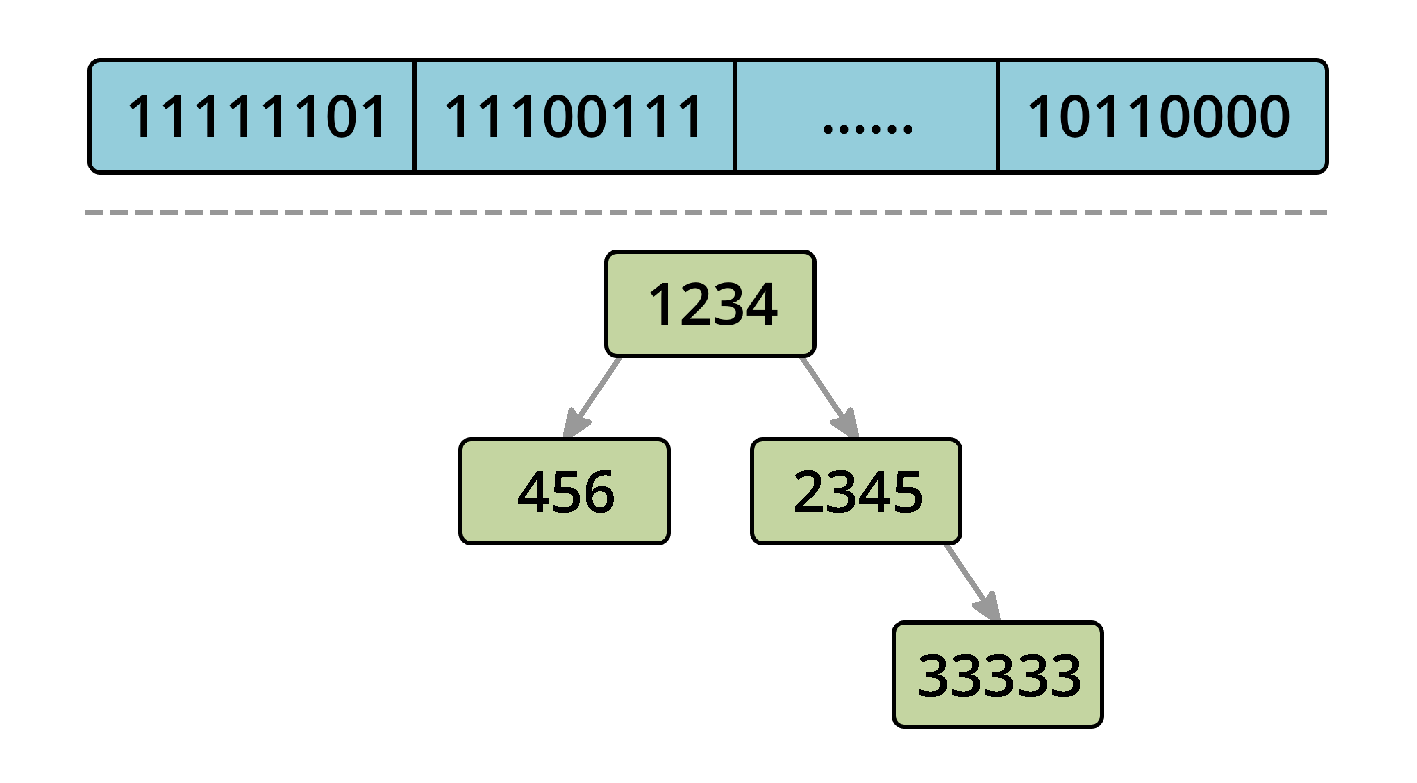
\includegraphics[width=0.9\linewidth]{figs/HybridDet.eps}
  \end{center}
  \vspace{-0.2cm}
  \caption{Hybrid Representation for Determinants.
  The occupancy of the most important orbitals is represented with bit-packing.
  The indices of the other occupied orbitals, which are 456, 1234, 2345, and 33333 in this case, are stored in a self-balancing binary search tree~\cite{wiki:redblacktree}.
  }
  \label{fig:hybrid}
\end{figure}

The usage of this hybrid structure gives us high performance and compact storage for both the small number of important orbitals and a large number of nonimportant orbitals.

\subsection{Orbital Momentum Conservation}
We solve HEG under a plane wave basis set and periodic boundary condition.
One property of this basis set is that each orbital have a specific momentum associated with it, and thus we can use momentum conservation to reduce the storage of the HCI double excitation helper lists.

First, we find all the possible differences between the momentum of two orbitals.
Let $M$ be the number of orbitals ($k$ points), then the number of distinct differences between them is also of order $O(M)$.
For an orbital $i$, we denote the momentum of that orbital to be $k_{i}$.
We use $p$ and $q$ to denote the pair of occupied orbitals during excitation, and $r$ and $s$ to denote the pair of unoccupied orbitals to which the electrons are excited.
Then we have $\mathbf{k}_p + k_q = k_r + k_s$.
For HEG, as shown in Appendix~\ref{app:heg}, $k_p - k_q$ and $k_p - k_r$ uniquely determines the magnitude of the Hamiltonian matrix element associated with excitation $pq\to rs$.
Hence, for each possible momentum difference $k_{pq}$, we associate with it a list of $\langle k_{pr}, |H_{pqrs}|\rangle$ pairs in descending order of $|H_{pqrs}|$.
Fig.~\ref{fig:helper} illustrates the structure of these helper lists.
Finally, when using these helper lists to find important connected determinants to a given reference determinant, we perform the following for each pair of occupied orbitals $p$ and $q$: we go through the list associated with $k_{pq} = k_p - k_q$ to get $k_{pr}$ until the corresponding $|H_{pqrs}|$ falls below a given threshold.
Using $k_{pr}$ and momentum conservation, we can easily get $r$ and $s$, and thus the connected determinant which satisfies the SHCI criteria.
\begin{figure}
  \begin{center}
  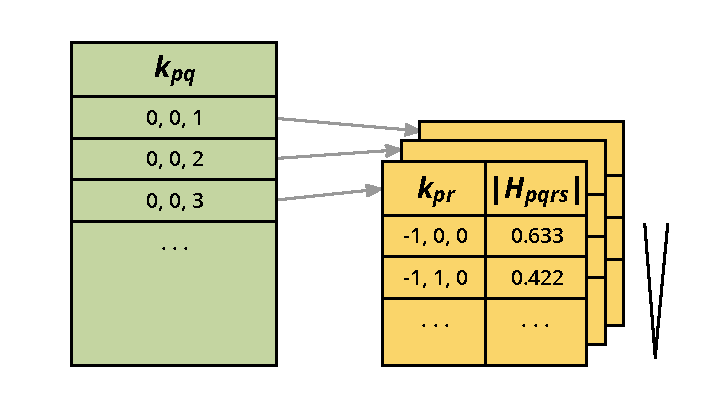
\includegraphics[width=0.9\linewidth]{figs/HelperList.eps}
  \end{center}
  \vspace{-0.2cm}
  \caption{SHCI Helper Lists for HEG.
  For each $k_{pq}$, we generate a list of $\langle k_{pr}, |H_{pqrs}|\rangle$ pairs and sort them into descending order of $|H_{pqrs}|$.
  When trying to find connected determinants from a given spawning determinant, we go through each occupied pair of orbitals $p$ and $q$, calculate their momentum difference $k_{pq}$, and go through the corresponding list until $|H_{pqrs}|$ falls below a certain threshold.
  For each entry that we go through in the list, we can obtain $r$ and $s$ by using $k_{pr}$ and momentum conservation.
  }
  \label{fig:helper}
\end{figure}

The storage complexity of these helper lists is $O(M^2)$, as opposed to $O(M^4)$ for chemistry systems.
The time complexity of finding determinants connected to a given determinant in descending order of importance is the same as in chemistry, which is $O(n_e^2 + n_D)$, where $n_e$ is the number of electrons and $n_D$ is the number of new determinants found.

%\section{Results}
\label{results}
We apply our revised algorithm to HEG of several different $r_s$ values in the mid to high density region and both the 14-electron and the 54-electron supercell sizes.
In each case, we calculate the correlation energies in several basis sets of different momentum cutoffs, and perform a complete basis set (CBS) extrapolation in the end.

We notice that when the electron density is high, the correlation energies depends significantly on the momentum cutoff.
Hence, in order to obtain more accurate results, we use up to 39,886 orbitals in our calculations.
In the high density region, this decreases the CBS extrapolation distance in previous literature by about more than an order of magnitude, and thus give us much shorter extrapolation distances and more accurate results.

\subsection{14-Electron Supercell}
\begin{figure}
  \begin{center}
  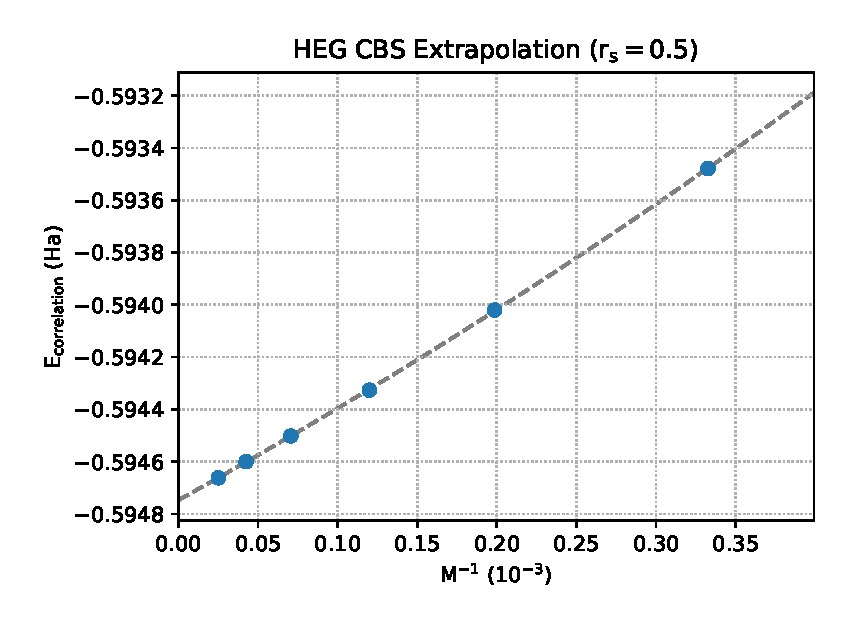
\includegraphics[width=\linewidth]{figs/cbs14e_05.eps}
  \end{center}
  \vspace{-0.2cm}
  \caption{Complete basis set extrapolation for HEG 14-electron supercell with $r_s=0.5$.
  The extrapolated correlation energy is $-0.594748(12)$~Ha.
  }
  \label{fig:cbs14e_05}
\end{figure}
\begin{figure}
  \begin{center}
  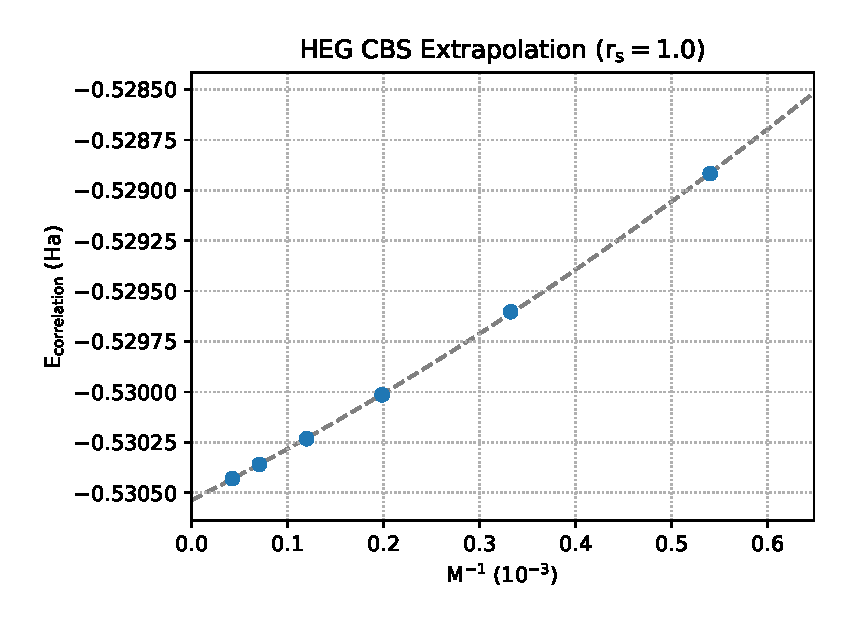
\includegraphics[width=\linewidth]{figs/cbs14e_10.eps}
  \end{center}
  \vspace{-0.2cm}
  \caption{Complete basis set extrapolation for HEG 14-electron supercell with $r_s=1.0$.
  The extrapolated correlation energy is $-0.530536(18)$~Ha.
  }
  \label{fig:cbs14e_10}
\end{figure}
\begin{figure}
  \begin{center}
  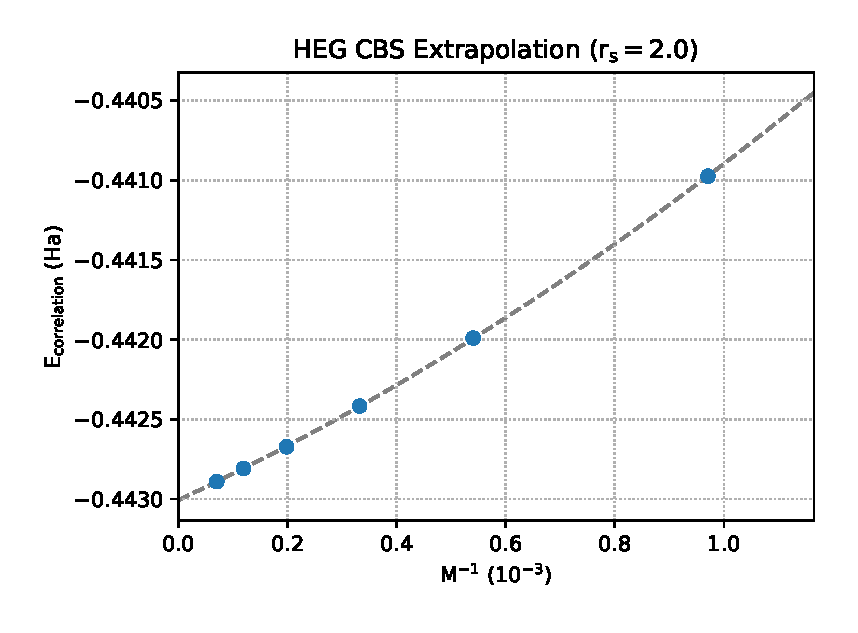
\includegraphics[width=\linewidth]{figs/cbs14e_20.eps}
  \end{center}
  \vspace{-0.2cm}
  \caption{Complete basis set extrapolation for HEG 14-electron supercell with $r_s=2.0$.
  The extrapolated correlation energy is $-0.443007(12)$~Ha.
  }
  \label{fig:cbs14e_20}
\end{figure}
\begin{figure}
  \begin{center}
  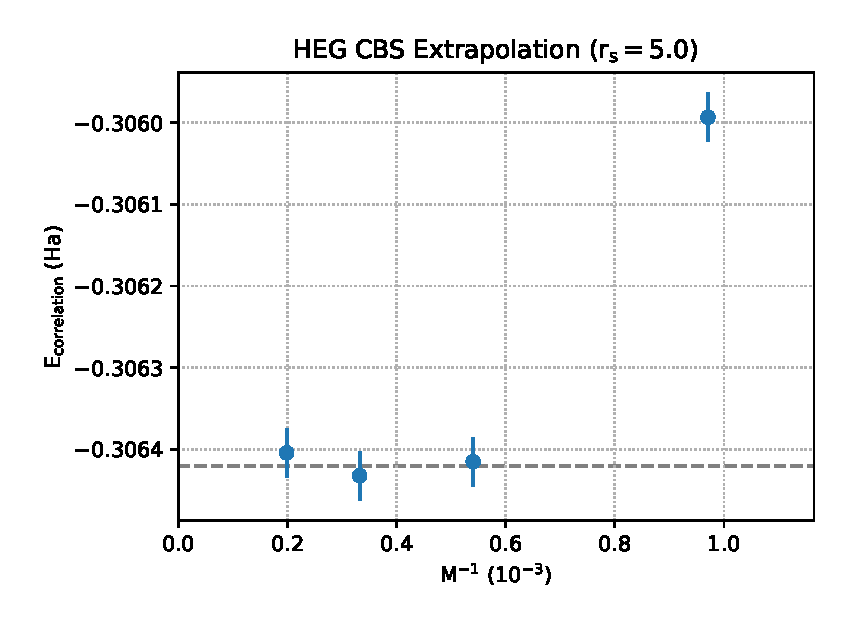
\includegraphics[width=\linewidth]{figs/cbs14e_50.eps}
  \end{center}
  \vspace{-0.2cm}
  \caption{Complete basis set extrapolation for HEG 14-electron supercell with $r_s=5.0$.
  Since the correlation energy is already converged after 2000 orbitals, we use the average of the last 3 points in this case.
  The extrapolated correlation energy is $-0.30642(5)$~Ha.
  }
  \label{fig:cbs14e_50}
\end{figure}
Fig.~\ref{fig:cbs14e_05} to \ref{fig:cbs14e_50} show our CBS extrapolation curves and Table~\ref{tab:results} reports our extrapolated correlation energies.
Here $M$ is the number of spin orbitals included in a plane wave basis set.

We use quadratic extrapolations weighted by $1/M$ for $r_s$ from 0.5 to 2.0.
For $r_s=5.0$, since it is already converged at the size of the basis sets that we use, we take the average of the last three points.
\begin{table}
\caption{Summary of the HEG Total Correlation Energies~(Ha).
CCMC~\cite{neufeld2017study} uses quantum Monte Carlo to evaluate coupled cluster wavefunctions with up to 1030 orbitals and 5\nth order excitation (CCSDTQ5).
FCIQMC~\cite{shepherd2012full} and its recent improvement FCIQMC-TC~\cite{luo2018combining} use up to 2368 orbitals.
SHCI uses up to 39886 orbitals, which give shorter extrapolation distances and much more accurate results than CCMC and FCIQMC.
}
\label{tab:results}
\begin{tabular}{| c || c || c | c | c | c |}
 \hline
 $r_s$ & SHCI & CCMC & FCIQMC & FCIQMC-TC \\
 \hline\hline
 0.5 & -0.594748(12) & -0.5947(2) & -0.5959(7) & -0.5948(2)\\
 \hline
 1.0 & -0.530536(18) & -0.5311(2) & -0.5316(4) & -0.5309(2)\\
 \hline
 2.0 & -0.443007(12) & -0.4434(10) & -0.444(1) & -0.4440(3)\\
 \hline
 5.0 & -0.30642(5) & -0.3025(4) & -0.307(1) & -0.3078(3)\\
 % DMC~\cite{rios2006inhomogeneous}
%  \hline
%  54 & 0.5 & -2.4316(6) & - & -2.435(7) & -2.387(2) \\
%  \hline
%  54 & 1.0 & -2.114(2) & - & -2.124(3) &  -2.125(2) \\
 \hline
\end{tabular}
\end{table}

We can see from this table that the results from SHCI are significantly more accurate than previous results.
This is mainly due to the fact that the high performance of SHCI and its capability to work with large basis sets enable us to go much closer to the infinite basis set. Fig.~\ref{fig:comparison} which plots the raw data points from FCIQMC~\cite{shepherd2012full} and SHCI, illustrates this.
\begin{figure}
  \begin{center}
  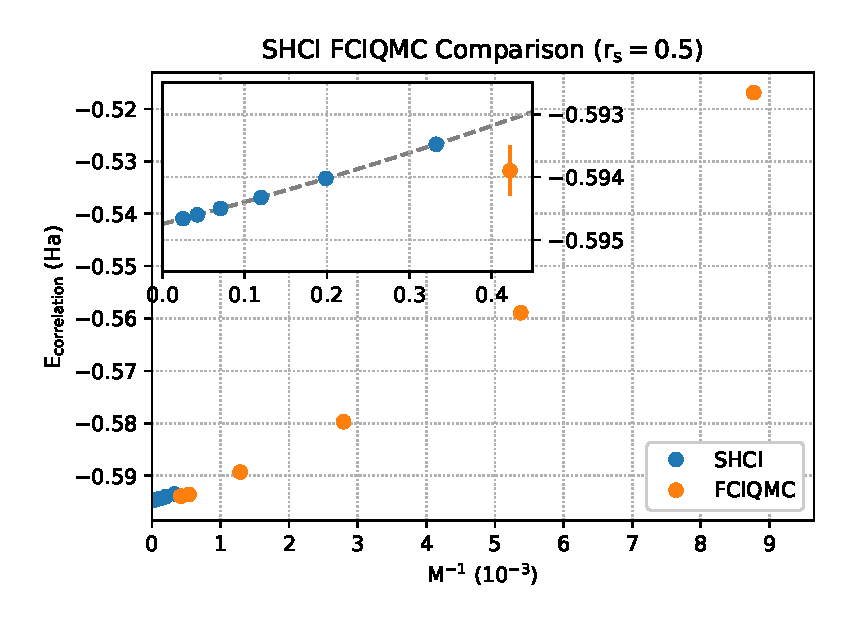
\includegraphics[width=\linewidth]{figs/compare.eps}
  \end{center}
  \vspace{-0.2cm}
  \caption{Comparison between SHCI results and FCIQMC results for $r_s=0.5$.
  Note that all the points have error bars smaller than the size of the points themselves except for the FCIQMC point on the zoomed-in view.
  SHCI goes much closer to the infinite basis set and thus achieves more accurate and reliable extrapolated results.
  }
  \label{fig:comparison}
\end{figure}

\subsection{54-Electron Supercell}
We also apply SHCI to the 54-electron supercell case.
Fig.~\ref{fig:cbs54e_05} shows the CBS extrapolation and Table~\ref{tab:results54} compares the SHCI results with FCIQMC and DMC.

We can see that our SHCI result agrees well with FCIQMC, but slighly lower than FCIQMC-TC, and all of them are much higher then BF-DMC, which probably used a poor trail wavefunction.
In these SHCI calculations, we use an order of magnitude more orbitals than FCIQMC and FCIQMC-TC, and the extrapolation distance of SHCI is about an order of magnitude smaller than FCIQMC and 4 times smaller than FCIQMC-TC.
Hence, we believe the extrapolated value from SHCI is likely to be more accurate and reliable than both FCIQMC and FCIQMC-TC.

\begin{figure}
  \begin{center}
  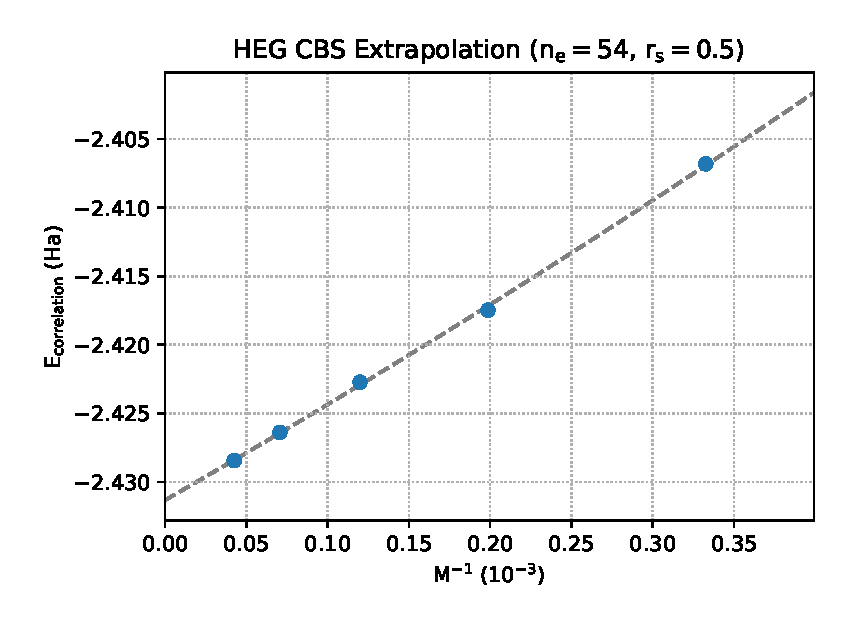
\includegraphics[width=\linewidth]{figs/cbs54e_05.eps}
  \end{center}
  \vspace{-0.2cm}
  \caption{Complete basis set extrapolation for HEG 54-electron supercell with $r_s=0.5$.
  The extrapolated correlation energy is $-2.4313(11)$~Ha.
  }
  \label{fig:cbs54e_05}
\end{figure}
\begin{table}
\caption{Summary of the HEG Total Correlation Energies~(Ha) with 54-Electron Supercells.
DMC~\cite{rios2006inhomogeneous} uses real space basis and backflow wave function.
FCIQMC~\cite{shepherd2012full} and its recent improvement FCIQMC-TC~\cite{luo2018combining} use up to 1850 orbitals.
SHCI uses up to 23506 orbitals, which give much shorter extrapolation distances than FCIQMC and thus more accurate results.
}
\label{tab:results54}
\begin{tabular}{| c || c || c | c | c | c |}
 \hline
 $r_s$ & SHCI & FCIQMC & FCIQMC-TC & BF-DMC \\
 \hline\hline
 0.5 & -2.4313(11) & -2.435(7) & -2.425(1) & -2.387(2) \\
 \hline
 % DMC~\cite{rios2006inhomogeneous}
%  \hline
%  54 & 0.5 & -2.4316(6) & - & -2.435(7) & -2.387(2) \\
%  \hline
%  54 & 1.0 & -2.114(2) & - & -2.124(3) &  -2.125(2) \\
 \hline
\end{tabular}
\end{table}
%\section{Conclusions}
In this paper, we apply our fast semistochastic heat-bath configuration interaction algorithm (SHCI) to the homongenous electron gas (HEG) problem in the mid to high density region.
The basis set incompleteness error is a dominating error in this region, and the uncertainty of the result depends a lot on the uncertainty of the extrapolation, which in terms depends on the extrapolation distance.
By using SHCI with up to 39886 orbitals, we reduce the extrapolation distance significantly and achieves more accurate results than state-of-the-art methods.

\label{conclusions}

\section{Introduction}
The homogeneous electron gas (HEG) is one of the most fundamental models in condensed-matter physics.
With a tunable parameter, the Wigner-Seitz radius $r_s$, controlling the density of the electrons,
the HEG provides a simple paradigm for studying interacting fermion problems
%of a wide range of systems from weakly correlated to strongly correlated.
ranging from weakly correlated to strongly correlated.
In addition, the HEG is a cornerstone of density functional theory (DFT).
%In the local density approximation (LDA), the local exchange-correlation energy $\epsilon_{xc}$ comes from HEG~\cite{perdew1986density, dahl2013local}. 
%And in the parametrization of more accurate exchange-correlation functionals, HEG energies are also used extensively~\cite{lundqvist2013theory}.
The exchange-correlation energy of the HEG is the entire exchange-correlation energy in the
local density approximation (LDA) of DFT, and it is an important component of more accurate exchange-correlation functionals~\cite{ParYan-BOOK-89,DreGro-BOOK-90}.

%The first accurate calculation of HEG ground state energies over a range of $r_s$ using \textit{ab initio} methods comes from the diffusion Monte Carlo (DMC)~\cite{ceperley1980ground}. However, due to the fixed-node approximation, the energies from DMC are not exact and depend heavily on the quality of the trial wavefunctions.
%Several attempts have successfully reduced the fixed-node error, but the question of the magnitude of the remaining errors and the new errors introduced by them has never been completely answered~\cite{kwon1998effects, rios2006inhomogeneous}.
The LDA is usually obtained from a fit to the diffusion Monte Carlo (DMC) exchange-correlation energy
per electron, $\epsilon_{xc}$, of the HEG with various $r_s$ values~\cite{CepAld-PRL-80}.
The DMC random walk is performed in real space (the coordinates of the electrons) and consequently
the computed energies are directly in the infinite-basis limit.
%However, DMC energies have an error due to the fixed-node approximation which depends on the
However, in order to control the Fermion sign problem, DMC is usually performed with the fixed-node approximation
and consequently the energies have a fixed-node error which depends on the
quality of the trial wavefunctions.
Backflow wavefunctions have been used to reduce the error~\cite{KwoCepMar-PRB-98,RioMaDruTowNee-PRE-06}
%Backflow wavefunctions have been used to reduce the error~\cite{RioMaDruTowNee-PRE-06}
but the magnitude of the remaining error is unclear.

%The full configuration interaction quantum Monte Carlo (FCIQMC) is another quantum Monte Carlo based method in the second quantized space. It stochastically samples the configuration space to approximate the full configuration interaction (FCI) energy at a reduced computational cost, and achieved a significantly and variationally lower energy for HEG $r_s=0.5$ than DMC~\cite{shepherd2012investigation}.
%However, FCIQMC has the basis set incompleteness error and requires a complete basis set (CBS) extrapolation, which in turn introduces an extrapolation error.
%In the mid-to-high density regime, the basis set incompleteness error dominates the total errors.
%For example, for HEG with $r_s=0.5$ and 14 electrons in each periodic box, the two largest FCIQMC calculations, which use 778 and 1850 orbitals and give $-0.5893(3)$~Ha and $-0.5936(3)$~Ha respectively, a $4.3$~mHa difference, which is much larger than the uncertainty of FCIQMC itself.
%Also, FCIQMC uses initiator approximation to skip side the Fermion-sign problem, which introduces the initiator error.
%This error can only be reduced by using a large number of walkers, thus also limits the accuracy.

%The coupled cluster Monte Carlo (CCMC) method with high excitation levels reproduces the results from FCIQMC for 14 electrons.
%It also shows that for HEG in the mid-to-high density regime, excitation levels all the way to four, i.e., CCSDTQ, are necessary to achieve comparable results as FCIQMC~\cite{neufeld2017study}.
%However, due to the high computational cost, CCSDTQ with CCMC has only been applied to 14 electrons and 358 orbitals.

In order to assess the magnitude of the DMC fixed-node error, other quantum Monte Carlo (QMC) methods
have been applied to the HEG.
In contrast to DMC, the random walk in the full configuration interaction quantum Monte Carlo (FCIQMC)
method~\cite{BooThoAla-JCP-09,CleBooAla-JCP-10,SheBooAla-JCP-12,SheBooGruAla-PRB-12} is in the space of
occupation numbers of a finite number of orbitals.
The finite basis set energies need to be extrapolated to obtain the complete basis set (CBS) energies.
The Fermion sign problem in FCIQMC is controlled by making an {\it initiator approximation}.
The initiator error disappears in the infinite walker population limit, and for many systems it is practical
to use a sufficiently large population to make the initiator error negligible.
In the mid-to-high density regime, the basis set incompleteness error is the dominant error.
For example, for the HEG with $r_s=0.5$ and 14 electrons in each periodic cell, the two largest FCIQMC
calculations, which use 778 and 1850 orbitals yield correlation energies $-0.5893(3)$~Ha and $-0.5936(3)$~Ha
respectively, a $4.3$~mHa difference, which is larger than the estimated initiator and statistical errors.

The coupled cluster Monte Carlo (CCMC) method~\cite{Tho-PRL-10,neufeld2017study} is closely related
to FCIQMC but yields coupled cluster energies in the infinite walker limit.
It has been used~\cite{neufeld2017study} to compute the correlation energy of the HEG with a 14-electron periodic cell for
$r_s$ in the range $0.5 - 5.0\ a_0$ with excitation orders up to five, i.e., CCSDTQ5, and 358 orbitals.
As expected high excitation orders are necessary to get agreement with FCIQMC at the larger $r_s$ values.

%The method that we use in this paper is a modified version of the recently proposed fast heat-bath configuration interaction (SHCI).
%SHCI is a selected configuration interaction plus perturbation method (SCI+PT) and distinguishes from other SCI+PT methods in that it uses precomputed double excitation lists to significantly improve the efficiency in both the variational stage and perturbation stage~\cite{holmes2016heat}.
%HCI in its original form requires a large amount of memory in the perturbation stage.
%The semistochastic heat-bath configuration interaction (SHCI) eliminates this memory bottleneck by performing stochastic perturbation on less important determinants~\cite{sharma2017semistochastic}.
%SHCI has several attractive features, such no sign problem, no autocorrelation, and it is usually faster than the original HCI if a stochastic error of 0.1 mHa is acceptable.
%Fast SHCI introduces the fast Hamiltonian generation algorithm and the 3-step perturbation algorithm, which further improve the efficiency of SHCI by more than an order of magnitude~\cite{li2018fast}.
%
%This paper adapts the SHCI algorithm to the homogeneous electron gas problem (HEG).
%We introduce a more space efficient data structure to deal with large basis sets.
%In addition, we optimize the storage and the usage of the double excitation lists, taking into consideration the mementum conservation property of the plane-wave based orbitals of HEG.
%Finally, we apply the revised algorithm to HEG with up to 39,886 orbitals, which is more than an order of magnitude larger than previously ever done with previous essentially exact methods.
%This reduces the extrapolation distances in the complete basis extrapolation significantly and thus gives more accurate and reliable results.

The method used in this paper is a modified version of the recently proposed heat-bath configuration interaction (SHCI) method~\cite{HolTubUmr-JCTC-16,ShaHolJeaAlaUmr-JCTC-17,LiOttHolShaUmr-JCP-18}.
SHCI is a selected configuration interaction plus perturbation method (SCI+PT) method.
It differs from SCI+PT methods in that it uses precomputed double excitation lists to avoid ever looking
at determinants that do not satisfy the threshold for contributing to the variational wavefunction
or the perturbative correction~\cite{HolTubUmr-JCTC-16}, and it evaluates the perturbative
correction semistochastically to avoid a memory bottleneck~\cite{ShaHolJeaAlaUmr-JCTC-17}.
Recently, SHCI has been sped up by another order of magnitude by introducing a fast Hamiltonian generation algorithm and replacing the 2-step semistochastic perturbative correction by a 3-step algorithm~\cite{LiOttHolShaUmr-JCP-18}.

This paper adapts the SHCI algorithm to the homogeneous electron gas problem (HEG).
We introduce a more space efficient data structure for representing determinants when using very
large basis sets.
In addition, we optimize the storage and the usage of the double excitation lists, taking into consideration the mementum conservation property of the plane-wave orbitals.
Finally, we apply the revised algorithm to the HEG with up to 39,886 orbitals, which is more than
an order of magnitude larger than previously used in methods that yield essentially exact energies within a basis,
in order to get accurate extrapolated energies in the complete basis limit.
%This reduces the extrapolation distances in the complete basis extrapolation significantly and thus gives more accurate and reliable results.

We organize this paper as follows:
In section \ref{SHCI}, we briefly review the SHCI algorithm and its recent improvements.
In section \ref{HEG}, we adapt SHCI to the homogeneous electron gas problem (HEG).
In section \ref{results}, we use the revised algorithm to obtain accurate HEG results in the mid-to-high density regime.
Section \ref{conclusions} concludes the paper.

\section{Fast Semistochastic Heat-Bath Configuration Interaction}
\label{SHCI}

The SHCI algorithm has two stages, the variational stage, and the perturbative stage.
In the following, we use $\V$ for the set of determinants in the variational wavefunction, and $\P$ for the determinants that contribute to the perturbative correction.

\subsection{Variational Stage}
%HCI starts with an initial set of determinants $\V_0$, usually just the Hartree-Fock determinant, and generates the variational wave function through an iterative process.
%
%In each iteration, we first try to find a set of new determinants $\V'$ that connects to the current determinants set $\V$.
%A new determinant $D_a$ is connected to a determinant in $\V$ if
%\beq
%\exists D_{i} \in \V, \; \mathrm{such\; that} \left|H_{ai} c_{i}\right| \ge \epsilon_{1}
%\eeq
%Where $c_i$ is the coefficient of determinant $D_i$ and $H_{ai}$ is the Hamiltonian matrix element between determinant $D_a$ and $D_i$.
%Then, we add the new determinants into $\V$, diagonalize and obtain the new lowest eigenvalue $E_{V}$ and eigenvector $\Psi _{V} = \sum _{D _{i} \in \V} c _{i} \left|D _{i}\right\rangle$.
%And when the change in $E_V$ falls below a certain threshold, we terminate the process.
%
%This process is similar to other selected-CI methods (SCI) but has a crucial difference in the selection criteria.
%Conventional SCI often use perturbation expressions as the criteria which are expensive to evaluate, such as the $\left|\frac{\sum _{i} H _{a i} c _{i}}{E _{0} - H _{a a}}\right| > \epsilon _{1}$ used in CIPSI \cite{huron1973iterative}.
%While HCI uses the much less expensive $\left|H _{a i} c _{i}\right| \ge \epsilon _{1}$ and new determinants meeting this criterion can be found very efficiently by looking up a few precomputed lists of double excitation matrix elements without evaluating the criterion \cite{holmes2016heat}.
%
%In addition, SHCI introduces the fast Hamiltonian construction algorithm, which speeds up the sparse Hamiltonian matrix construction by an order of magnitude~\cite{li2018fast}.

Starting from an initial set of determinants, usually just a single determinant (e.g. the Hartree-Fock determinant,
or a determinant of natural orbitals, or a determinant of optimized orbitals),
the SHCI method generates the variational wavefunction using an iterative process.
Indexing the determinants already in $\V$ by $i$ and those connected to those in $\V$ but not in $\V$ by $a$,
we add to $\V$ those determinants $D_a$ that satisfy the {\it HCI criterion}
\beq
\exists D_{i} \in \V, \; \mathrm{such\; that} \left|H_{ai} c_{i}\right| \ge \epsilon_{1},
\label{eq:hci_criterion}
\eeq
where $c_i$ is the coefficient of determinant $D_i$ and $H_{ai}$ is the Hamiltonian matrix element between determinant $D_a$ and $D_i$.
The Hamiltonian is constructed in the expanded set of determinants in $\V$ and diagonalized to obtain the new lowest eigenvalue $E_{V}$ and eigenvector $\Psi _{V} = \sum _{D _{i} \in \V} c _{i} \left|D _{i}\right\rangle$.
When the change in $E_V$ falls below a certain threshold, the process is terminated.

This process is similar to that in other selected-CI methods (SCI) but has a crucial difference in the selection criteria.
Other SCI methods, e.g., CIPSI ~\cite{HurMalRan-JCP-73}, use a perturbative criterion, e.g.,
\beq
\left|\frac{\sum_{i} H_{ai} c_{i}}{E_{0} - H_{aa}}\right| > \epsilon_{1}.
\label{eq:cipsi_criterion}
\eeq
The advantages of the HCI criterion of Eq.~\ref{eq:hci_criterion} are that the sum in the numerator, and the diagonal matrix
element in the denominator of Eq.~\ref{eq:cipsi_criterion} do not need to be computed, and, most importantly that by
precomputing sorted lists of double-excitation matrix elements it is possible to exit the loops over connected determinants
as soon as the HCI criterion is violated.
In addition, we have recently introduced a fast Hamiltonian construction algorithm~\cite{LiOttHolShaUmr-JCP-18}, which speeds up the sparse Hamiltonian matrix construction by an order of magnitude.

\subsection{Perturbative Stage}
%The second order perturbative correction is
%\beq
%\Delta E_2^{(\mathrm{d})} &=& \sum _{D _{a} \in \P} \frac{\left(\sum _{D _{i} \in \V} H _{a i} c _{i}\right) ^{2}}{E _{V} - H _{a a}}
%\eeq
%where the sum is over determinants in the perturbative space, $\P$, i.e. determinants that are connected to
%those in $\V$ but not in $\V$.
%HCI makes an additional approximation and includes only those $H_{ai}c_{i}$ terms when
%\beq
%\exists D _{i} \in \V , \mathrm{s . t .} \left|H _{a i} c _{i}\right| \ge \epsilon _{2}
%\eeq
%This criterion allows us to use similar techniques as the variational stage to find the connected determinants using precomputed lists without wasting time on determinants that do not meet the criterion \cite{holmes2016heat}.
%
%We refer to the method above as the deterministic perturbation and it requires storing the entire perturbation space $\P$, which causes a memory bottleneck.
%This bottleneck can be eliminated by the semistochastic perturbation algorithm~\cite{sharma2017semistochastic}.
%The combined perturbation correction is 
%\beq
%\Delta E _{2} \left(\epsilon _{2}\right) = \left[\Delta E _{2} ^{\left(\mathrm{s}\right)} \left(\epsilon _{2} \right) - \Delta E _{2} ^{\left(\mathrm{s}\right)} \left(\epsilon _{2} ^{\left(\mathrm{d}\right)}\right)\right] + \Delta E _{2} ^{\left(\mathrm{d}\right)} \left(\epsilon _{2} ^{\left(\mathrm{d}\right)}\right)
%\eeq
%where $\epsilon _{2} ^{\left(\mathrm{d}\right)}$ is the deterministic $\epsilon_2$, which can be much larger than the targeting $\epsilon_2$.
%$\Delta E _{2} ^{\left(\mathrm{s}\right)}$ is the stochastic perturbation correction
%\begin{align*}
%\Delta E _{2} ^{\left(\mathrm{s}\right)} = & \frac{1}{N _{d} \left(N _{d} - 1\right)} \left\langle \sum _{D _{a} \in \P} \left[\left(\sum _{i} ^{N _{d} ^{\mathrm{( d i f f )}}} \frac{w _{i} c _{i} H _{a i}}{p _{i}}\right) ^{2} \right. \right. \\ + 
% & \left. \left. \sum _{i} ^{N _{d} ^{\mathrm{( d i f f )}}} \left(\frac{w _{i} \left(N _{d} - 1\right)}{p _{i}} - \frac{w _{i} ^{2}}{p _{i} ^{2}}\right) c _{i} ^{2} H _{a i} ^{2}\right] \frac{1}{E _{0} - E _{a}} \right\rangle
%\end{align*}
%Here $N_d$ is the number of determinants in a sample and $N_d^{\mathrm{(diff)}}$ is the number unique ones.
%$p_i$ and $w_i$ are the probability of selecting determinant $D_i$ and the number of repeats respectively.
%And new determinants are sampled with a finite discrete probability distribution $p _{i} = \frac{\left|c _{i}\right|}{\sum \left|c _{i}\right|}$, which has no sign problem or autocorrelation at all.
%
%We further introduce the 3-step batch perturbation to improve the speed of the perturbative stage.
%Batch perturbation divides the perturbative space into batches and evaluates the perturbative corrections batch by batch.
%This allows us to use much smaller $\epsilon_2^{(d)}$ and much larger $N_d$, both of which give superlinear speedup.
%We also insert a new pseudostochastic step between the original deterministic step and the stochastic step.
%This psedostochastic step evaluates the deterministic perturbation expression in batches, and stops early when the uncertainty of the energy drops below a certain threshold.
%Overall, the 3-step batch perturbation algorithm speeds up perturbative calculations by more than an order of magnitude, and enable us to include the entire Hilbert space during the perturbative stage ($\epsilon_2=0$)~\cite{li2018fast}.


%We employ a 3-step semistochastic perturbation theory~\cite{LiOttHolShaUmr-JCP-18}.
%The total deterministic correction is simply the sum of the corrections from all the batches
The perturbative correction is
\beq
%$$\Delta E_{2}^{(d)} \left(\epsilon \right) = \sum_ {B} \sum_{D_{a}} \frac{\left(\sum_{D_i \in \V, \left|H_{a i} c_{i}\right| \ge \epsilon_{2}, h(D_a)\in B} H_{a i} c_{i}\right) ^{2}}{E_{V} - H_{a a}}$$
%$$\Delta E_{2} \left(\epsilon^{\rm det} \right) = \sum_{B} \sum_{D_a \in \P, h(D_a)\in B} \frac{\left(\sum^{(\epsilon_{2}^{\rm det})}_{D_i \in \V} H_{a i} c_{i}\right) ^{2}}{E_{V} - H_{a a}}$$
\Delta E_{2} \left(\epsilon_2\right) = \sum_{\substack{D_a \in \P}} \frac{\left(\sum^{(\epsilon_2)}_{D_i \in \V} H_{a i} c_{i}\right) ^{2}}{E_{V} - H_{aa}}
\eeq
where the sum includes only those determinants that meet the criterion $\left|H_{ai} c_{i}\right| \ge \epsilon_{2}$, with $\epsilon_{2} \ll \epsilon_{1}$.
This allows us to use precomputed lists, just as in the variational stage, to avoid wasting time on determinants that do not meet the criterion~\cite{HolTubUmr-JCTC-16}.
However, the number of perturbative determinants, indexed by $a$, is orders of magnitude larger than the number of variational determinants and this creates
a severe memory bottleneck.

To overcome this, we employ a 3-step semistochastic perturbation theory~\cite{LiOttHolShaUmr-JCP-18}, wherein the total perturbative correction is
\beq
\Delta E_{2} \left(\epsilon_{2}\right) &=& 
  \left[\Delta E_{2}^{\mathrm{sto}} \left(\epsilon_{2} \right) - \Delta E_{2}^{\mathrm{sto}} \left(\epsilon_{2}^{\rm psto}\right)\right] \nonumber \\
&+& \left[\Delta E_{2}^{\mathrm{psto}} \left(\epsilon_{2}^{\rm psto} \right) - \Delta E_{2}^{\mathrm{psto}} \left(\epsilon_{2}^{\rm dtm}\right)\right] \nonumber \\
&+& \Delta E_{2} ^{\mathrm{dtm}} \left(\epsilon_{2} ^{\mathrm{dtm}}\right)
\label{eq:semistoch_3-step_PT}
\eeq
where $\epsilon_{2} \ll \epsilon_{2}^{\rm psto} \ll \epsilon_{2}^{\rm dtm} \ll \epsilon_{1}$.
The determinants that satisfy $\epsilon_{1} > \left|H_{ai} c_{i}\right| \ge \epsilon_{2}^{\rm dtm}$ are included deterministically, i.e., all
the variational and perturbative determinants that satisfy this condition are summed over,
the determinants that satisfy $\epsilon_{2}^{\rm dtm} > \left|H_{ai} c_{i}\right| \ge \epsilon_{2}^{\rm psto}$ are included pseudostochastically, i.e., all
the variational determinants but only a sampling of perturbative determinants that satisfy this condition are summed over, and,
the determinants that satisfy $\epsilon_{2}^{\rm psto} > \left|H_{ai} c_{i}\right| \ge \epsilon_{2}$ are included stochastically, i.e., both
the variational determinants and the perturbative determinants are sampled.
The variational determinants are sampled with probability
\beq
p_i = \frac{|c_i|}{\sum_i |c_i|},
\eeq
using the Alias method~\cite{walker1977efficient,kronmal1979alias}.
An unbiased estimator for $\Delta E_{2}$, using samples of $\Nd$ determinants, is~\cite{ShaHolJeaAlaUmr-JCTC-17},
\begin{widetext}
\begin{align}
\Delta E_{2}
%=& \sum_{a} \frac{1}{E_0 - E_a}\left[\sum_{ij}^{\V} H_{ai}H_{aj} c_ic_j\right]\nonumber\\
%=& \sum_{a} \frac{1}{E_0 - E_a}\left[\sum_{i\neq j}^{\V} H_{ai}H_{aj} c_ic_j + \sum_{i}^{\V} H_{ai}^2 c_i^2\right]\nonumber\\
%=& \left\langle \sum_{a} \frac{1}{E_0 - E_a}\left[\sum_{i\neq j}^{\Nddiff} \frac{w_i w_j c_ic_j H_{ai}H_{aj}}{\langle w_i w_j \rangle} + \sum_{i}^{\Nddiff} \frac{w_i c_i^2 H_{ai}^2}{\langle w_i \rangle}\right] \right\rangle \nonumber\\
%=& \left\langle \sum_{a} \frac{1}{E_0 - E_a}\left[\sum_{i\neq j}^{\Nddiff} \frac{w_i w_j c_ic_j H_{ai}H_{aj}}{p_ip_j\Nd(\Nd-1)} + \sum_{i}^{\Nddiff} \frac{w_i c_i^2 H_{ai}^2}{p_i\Nd}\right] \right\rangle \nonumber\\
%=& \left\langle \sum_{a} \frac{1}{E_0 - E_a}\left[{1 \over \Nd(\Nd-1)}\left\{\left(\sum_{i}^{\Nddiff} \frac{w_i c_i H_{ai}}{p_i}\right) \left(\sum_{j}^{\Nddiff} \frac{w_j c_j H_{aj}}{p_j}\right) - \sum_{i}^{\Nddiff} \frac{w_i^2 c_i^2 H_{ai}^2}{p_i^2}\right\}  + \sum_{i}^{\Nddiff} \frac{w_i c_i^2 H_{ai}^2}{p_i\Nd}\right]\nonumber \right\rangle \\
=& \frac{1}{\Nd(\Nd-1)} \left\langle \sum_{a} \frac{1}{E_0 - E_a} \left[\left(\sum_{i}^{\Nddiff} \frac{ w_i  c_i H_{ai}}{p_i}\right)^2  +\sum_{i}^{\Nddiff} \left(\frac{w_i(\Nd-1)}{p_i } - \frac{ w_i^2}{p_i^2}\right)c_i^2 H_{ai}^2\right] \right\rangle,
\label{eq:stofinal}
\end{align}
\end{widetext}

\section{Revision for Homogeneous Electron Gas}
\label{HEG}

In this section, we describe how we adapt our SHCI algorithm (previously used for chemical systems) to treat the HEG at mid to high densities.
The adaptations are necessitated by the use of a plane wave basis and the large number of orbitals
required for an accurate extrapolation to the complete basis limit.
Appendix~\ref{app:heg} gives the Hamiltonian matrix elements of HEG.

\subsection{Large Basis Set}
%In the mid to high density region, the correlation energy obtained from a finite basis set depends significantly on the size of the basis set.
%Hence, in order to achieve high accuracy for the infinite basis set, we have to use a large number of orbitals, which is one to two orders of magnitude larger than what SHCI calculations used.

The usual representation of determinants involves using bit-packing, i.e., one bits denote occupied orbitals
and zero bits denote unoccupied orbitals.  This becomes inefficient when the number of orbitals is much
larger than the number of electrons.
%To reduce storage and improve speed when using a large basis set, we introduce a new way for representing the determinants.
To reduce memory and time requirements when using a large basis set, we introduce a hybrid representation of the determinants.
First, the orbitals are sorted into descending order of importance (occupancy).
%Then, we use bit-packing to represent the occupancy of the first few orbitals, which are the most important ones and mostly occupied, and use a self-balancing binary search tree~\cite{wiki:binarysearchtree}, called red-black tree~\cite{wiki:redblacktree}, to store the indices of the other occupied orbitals.
Then, bit-packing is used to represent the occupancy of the first few orbitals, and a self-balancing binary search tree~\cite{wiki:binarysearchtree}, namely a red-black tree~\cite{wiki:redblacktree}, is used to store the indices of the remaining orbitals.
Fig.~\ref{fig:hybrid} illustrates this hybrid structure.

The red-black tree is a common data structure for storing a set of distinct objects, which in our case are the indices of the occupied orbitals.
An excitation corresponds to a deletion of one or two occupied orbitals and insertion of one or two unoccupied orbitals.
The worst case time complexity for this operation on a red-black tree (including the cost of rebalancing the tree) is $O(\log N)$.
Another common operation on determinants is going through the occupied orbitals in order, which corresponds to an inorder traversal~\cite{wiki:treetraversal} of the tree.
The time complexity of this traversal is $O(N)$.
%, which makes it a better choice than a hash table.
\begin{figure}
  \begin{center}
  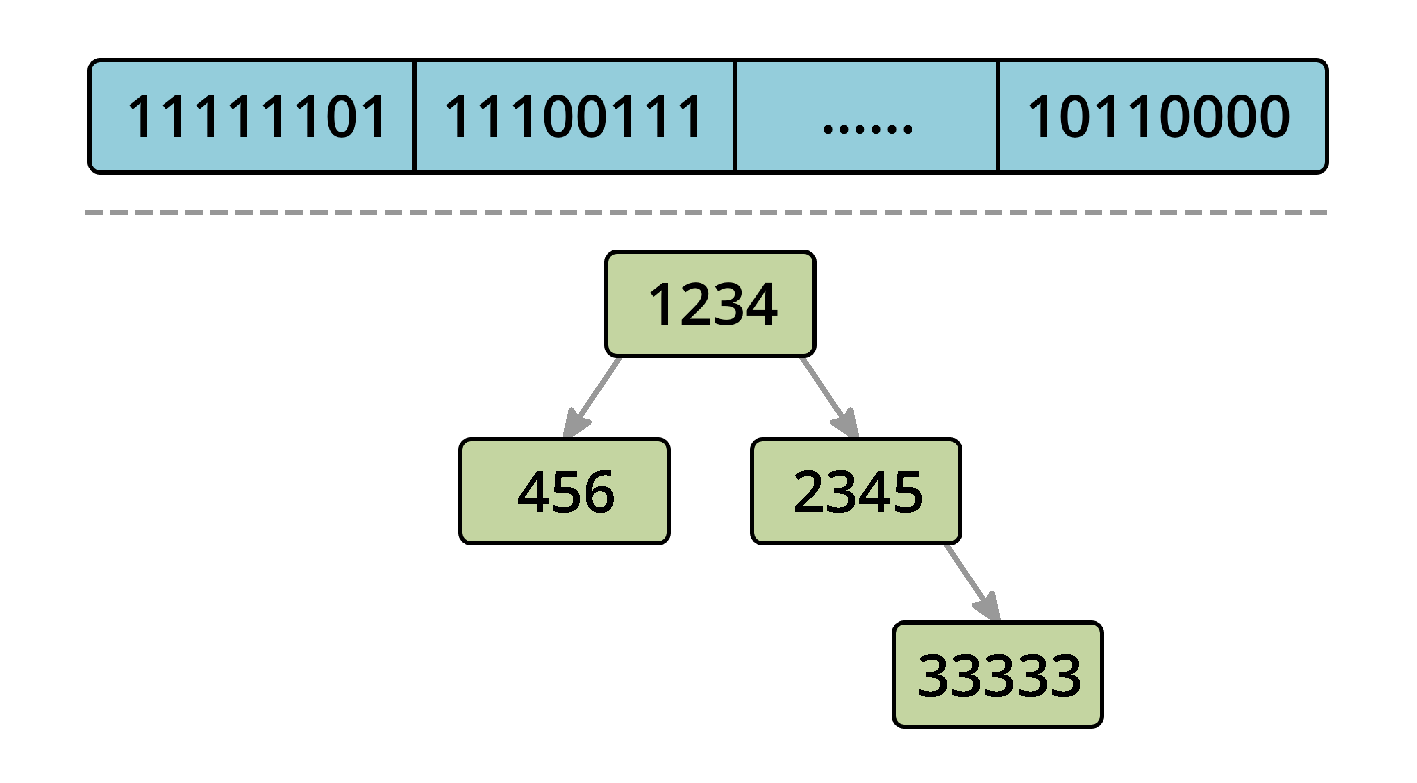
\includegraphics[width=0.9\linewidth]{figs/HybridDet.eps}
  \end{center}
  \vspace{-0.2cm}
  \caption{Hybrid Representation for Determinants.
  The occupancy of the most important orbitals is represented with bit-packing.
  The indices of the other occupied orbitals, which are 456, 1234, 2345, and 33333 in this case, are stored in a self-balancing binary search tree~\cite{wiki:redblacktree}.
  }
  \label{fig:hybrid}
\end{figure}
This hybrid structure gives us high performance and compact storage when there are a small number of important orbitals and a large number of unimportant orbitals.

\subsection{Orbital Momentum Conservation}
%We solve HEG under a plane wave basis set and periodic boundary condition.
%One property of this basis set is that each orbital have a specific momentum associated with it, and thus we can use momentum conservation to reduce the storage of the HCI double excitation helper lists.
We employ a plane wave basis set and periodic boundary conditions.
Since the orbitals are momentum eigenstates, momentum conservation can be used
to reduce the storage of the HCI double excitation helper lists.

First, we find all the possible differences between the momenta of two orbitals.
Let $M$ be the number of orbitals ($\mathbf{k}$ points), then the number of distinct differences between them is also of order $O(M)$.
For an orbital $i$, we denote the momentum of that orbital to be $\mathbf{k}_{i}$.
We use $p$ and $q$ to denote the pair of occupied orbitals during excitation, and $r$ and $s$ to denote the pair of unoccupied orbitals to which the electrons are excited.
Then we have $\mathbf{k}_p + \mathbf{k}_q = \mathbf{k}_r + \mathbf{k}_s$.
For HEG, as shown in Appendix~\ref{app:heg}, $\mathbf{k}_p - \mathbf{k}_q$ and $\mathbf{k}_p - \mathbf{k}_r$ uniquely determines the magnitude of the Hamiltonian matrix element associated with excitation $pq\to rs$.
Hence, for each possible momentum difference $\mathbf{k}_{pq}$, we associate with it a list of $\langle \mathbf{k}_{pr}, |H_{pqrs}|\rangle$ pairs in descending order of $|H_{pqrs}|$.
Fig.~\ref{fig:helper} illustrates the structure of these helper lists.
Finally, when using these helper lists to find important connected determinants to a given reference determinant, we perform the following for each pair of occupied orbitals $p$ and $q$: we go through the list associated with $\mathbf{k}_{pq} = \mathbf{k}_p - \mathbf{k}_q$ to get $\mathbf{k}_{pr}$ until the corresponding $|H_{pqrs}|$ falls below a given threshold.
Using $\mathbf{k}_{pr}$ and momentum conservation, we can easily get $r$ and $s$, and thus the connected determinant which satisfies the SHCI criteria.
\begin{figure}
  \begin{center}
  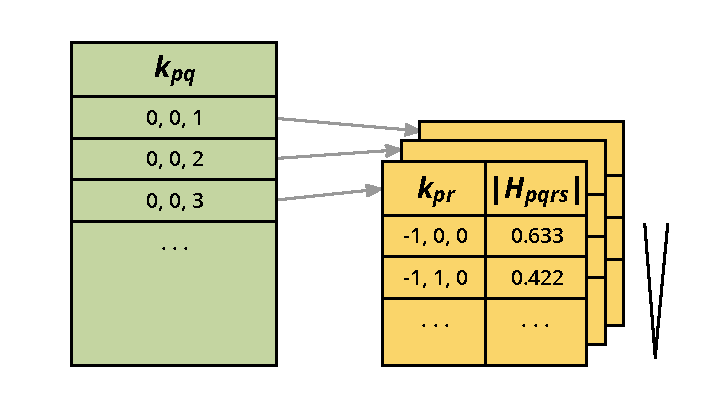
\includegraphics[width=0.9\linewidth]{figs/HelperList.eps}
  \end{center}
  \vspace{-0.2cm}
  \caption{SHCI Helper Lists for HEG.
  For each $\mathbf{k}_{pq}$, we generate a list of $\langle \mathbf{k}_{pr}, |H_{pqrs}|\rangle$ pairs and sort them in descending order of $|H_{pqrs}|$.
  When trying to find connected determinants from a given spawning determinant, we go through each occupied pair of orbitals $p$ and $q$, calculate their momentum difference $\mathbf{k}_{pq}$, and go through the corresponding list until $|H_{pqrs}|$ falls below a certain threshold.
  For each entry that we go through in the list, we can obtain $r$ and $s$ by using $\mathbf{k}_{pr}$ and momentum conservation.
  }
  \label{fig:helper}
\end{figure}

The storage complexity of these helper lists is $O(M^2)$, as opposed to $O(M^4)$ for chemistry systems.
The time complexity of finding determinants connected to a given determinant in descending order of importance is the same as in chemistry, which is $O(n_e^2 + n_D)$, where $n_e$ is the number of electrons and $n_D$ is the number of new determinants found.

\section{Results}
\label{results}
We apply our revised algorithm to HEG of several different $r_s$ values in the mid to high density region and both 14-electron and 54-electron supercells.
In each case, we calculate the correlation energies in several basis sets of different momentum cutoffs, and perform a complete basis set (CBS) extrapolation.

When the electron density is high, the correlation energies depend significantly on the momentum cutoff.
Hence, in order to obtain more accurate results, we use up to 39,886 orbitals in our calculations.
In the high density region, this decreases the CBS extrapolation distance in previous literature by about more than an order of magnitude, and thus give us much shorter extrapolation distances and more accurate results.

\subsection{14-Electron Supercell}
\begin{figure}
  \begin{center}
  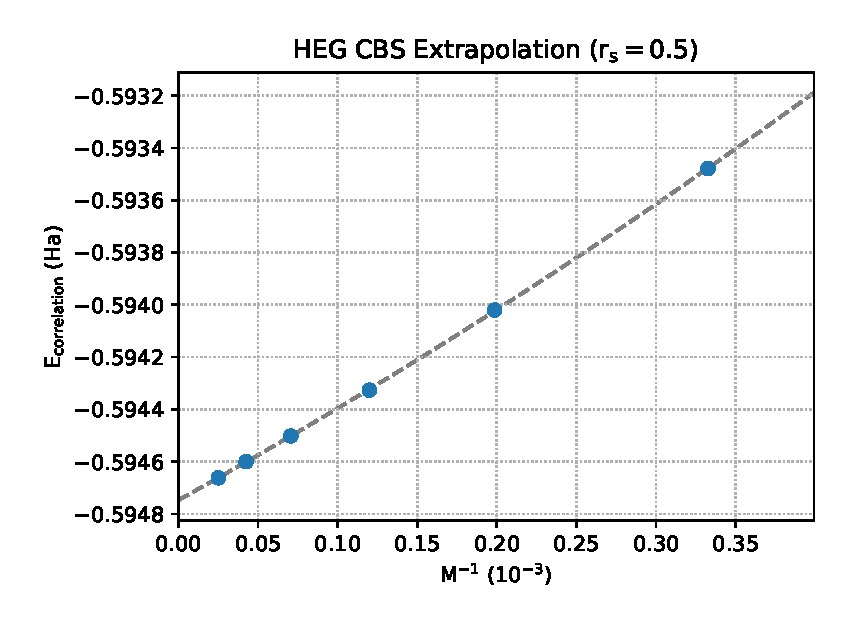
\includegraphics[width=\linewidth]{figs/cbs14e_05.eps}
  \end{center}
  \vspace{-0.2cm}
  \caption{Complete basis set extrapolation for HEG 14-electron supercell with $r_s=0.5$.
  The extrapolated correlation energy is $-0.594748(12)$~Ha.
  }
  \label{fig:cbs14e_05}
\end{figure}
\begin{figure}
  \begin{center}
  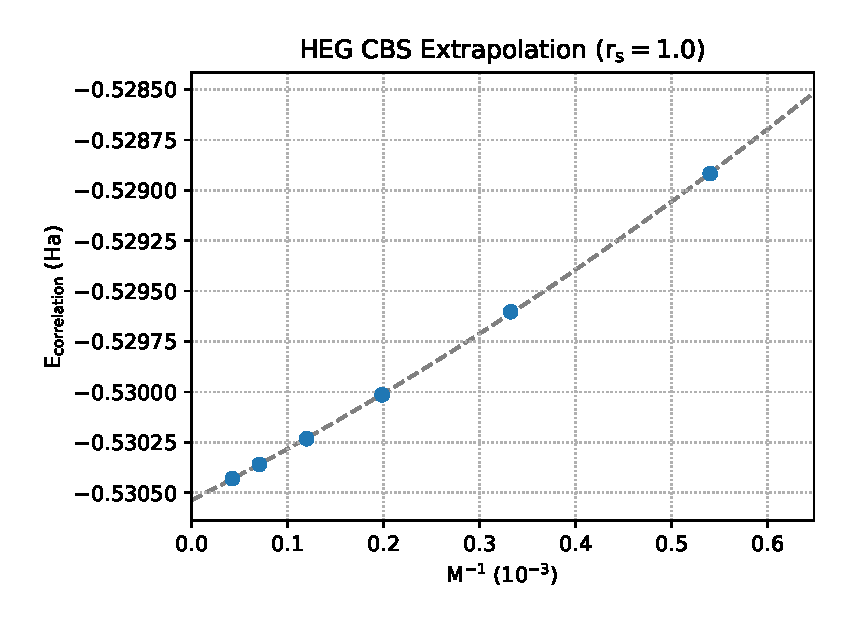
\includegraphics[width=\linewidth]{figs/cbs14e_10.eps}
  \end{center}
  \vspace{-0.2cm}
  \caption{Complete basis set extrapolation for HEG 14-electron supercell with $r_s=1.0$.
  The extrapolated correlation energy is $-0.530536(18)$~Ha.
  }
  \label{fig:cbs14e_10}
\end{figure}
\begin{figure}
  \begin{center}
  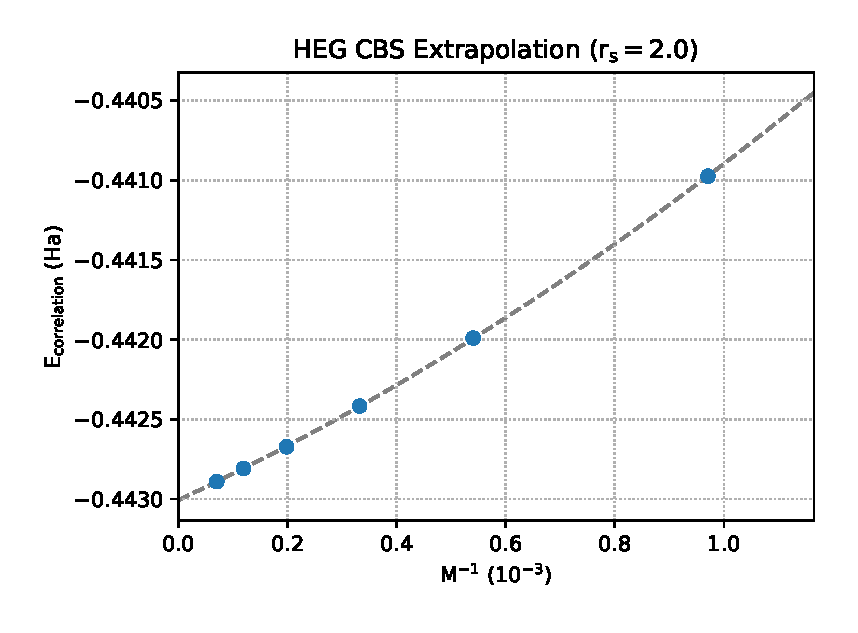
\includegraphics[width=\linewidth]{figs/cbs14e_20.eps}
  \end{center}
  \vspace{-0.2cm}
  \caption{Complete basis set extrapolation for HEG 14-electron supercell with $r_s=2.0$.
  The extrapolated correlation energy is $-0.443007(12)$~Ha.
  }
  \label{fig:cbs14e_20}
\end{figure}
\begin{figure}
  \begin{center}
  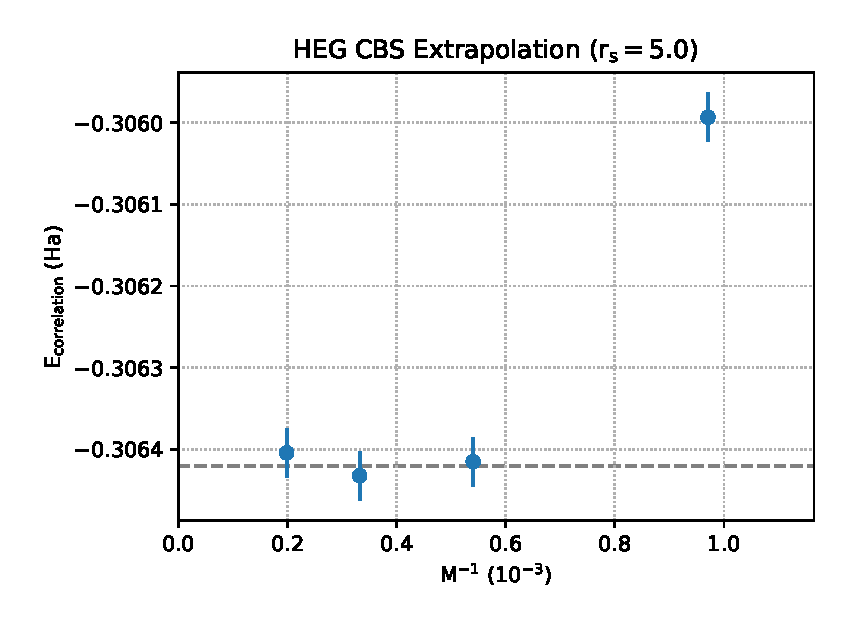
\includegraphics[width=\linewidth]{figs/cbs14e_50.eps}
  \end{center}
  \vspace{-0.2cm}
  \caption{Complete basis set extrapolation for HEG 14-electron supercell with $r_s=5.0$.
  Since the correlation energy is already converged after 2000 orbitals, we use the average of the last 3 points in this case.
  The extrapolated correlation energy is $-0.30642(5)$~Ha.
  }
  \label{fig:cbs14e_50}
\end{figure}
Fig.~\ref{fig:cbs14e_05} to \ref{fig:cbs14e_50} show our CBS extrapolation curves and Table~\ref{tab:results} reports our extrapolated correlation energies.
Here $M$ is the number of spin orbitals included in a plane wave basis set.

We use quadratic extrapolations weighted by $1/M$ for $r_s$ from 0.5 to 2.0.
For $r_s=5.0$, since it is already converged at the size of the basis sets that we use, we take the average of the last three points.
\begin{table}
\caption{Summary of the HEG Total Correlation Energies~(Ha).
CCMC~\cite{neufeld2017study} uses quantum Monte Carlo to evaluate coupled cluster wavefunctions with up to 1030 orbitals and 5\nth order excitation (CCSDTQ5).
FCIQMC~\cite{shepherd2012full} and its recent improvement FCIQMC-TC~\cite{luo2018combining} use up to 2368 orbitals.
SHCI uses up to 39886 orbitals, which give shorter extrapolation distances and much more accurate results than CCMC and FCIQMC.
}
\label{tab:results}
\begin{tabular}{| c || c || c | c | c | c |}
 \hline
 $r_s$ & SHCI & CCMC & FCIQMC & FCIQMC-TC \\
 \hline\hline
 0.5 & -0.594748(12) & -0.5947(2) & -0.5959(7) & -0.5948(2)\\
 \hline
 1.0 & -0.530536(18) & -0.5311(2) & -0.5316(4) & -0.5309(2)\\
 \hline
 2.0 & -0.443007(12) & -0.4434(10) & -0.444(1) & -0.4440(3)\\
 \hline
 5.0 & -0.30642(5) & -0.3025(4) & -0.307(1) & -0.3078(3)\\
 % DMC~\cite{rios2006inhomogeneous}
%  \hline
%  54 & 0.5 & -2.4316(6) & - & -2.435(7) & -2.387(2) \\
%  \hline
%  54 & 1.0 & -2.114(2) & - & -2.124(3) &  -2.125(2) \\
 \hline
\end{tabular}
\end{table}

We can see from this table that the results from SHCI are significantly more accurate than previous results.
This is mainly due to the fact that the high performance of SHCI and its capability to work with large basis sets enable us to go much closer to the infinite basis set. Fig.~\ref{fig:comparison} which plots the raw data points from FCIQMC~\cite{shepherd2012full} and SHCI, illustrates this.
\begin{figure}
  \begin{center}
  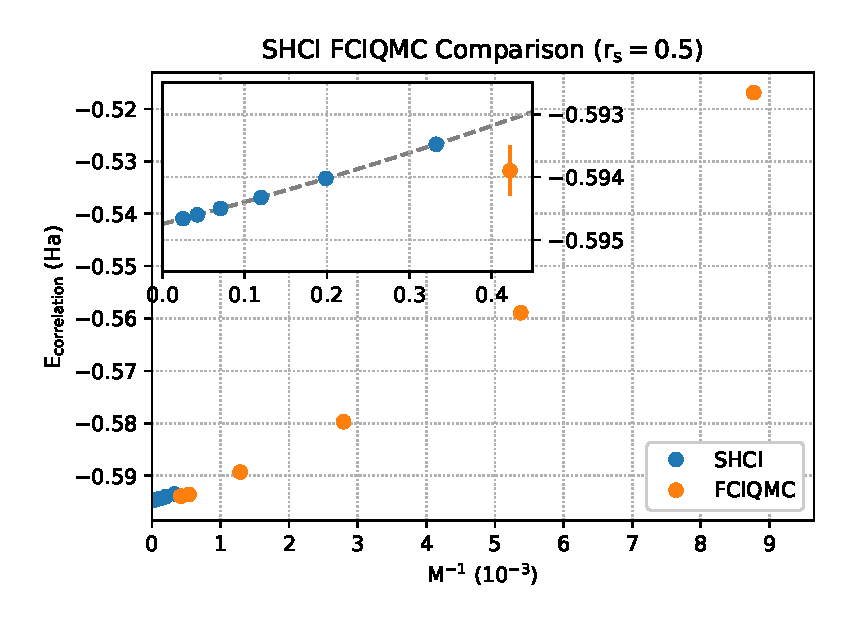
\includegraphics[width=\linewidth]{figs/compare.eps}
  \end{center}
  \vspace{-0.2cm}
  \caption{Comparison between SHCI results and FCIQMC results for $r_s=0.5$.
  Note that all the points have error bars smaller than the size of the points themselves except for the FCIQMC point on the zoomed-in view.
  SHCI goes much closer to the infinite basis set and thus achieves more accurate and reliable extrapolated results.
  }
  \label{fig:comparison}
\end{figure}

\subsection{54-Electron Supercell}
We also apply SHCI to the 54-electron supercell case.
Fig.~\ref{fig:cbs54e_05} shows the CBS extrapolation and Table~\ref{tab:results54} compares the SHCI results with FCIQMC and DMC.

We can see that our SHCI result agrees well with FCIQMC, but slighly lower than FCIQMC-TC, and all of them are much higher then BF-DMC, which probably used a poor trial wavefunction.
In these SHCI calculations, we use an order of magnitude more orbitals than FCIQMC and FCIQMC-TC, and the extrapolation distance of SHCI is about an order of magnitude smaller than FCIQMC and 4 times smaller than FCIQMC-TC.
Hence, we believe the extrapolated value from SHCI is likely to be more accurate and reliable than both FCIQMC and FCIQMC-TC.

\begin{figure}
  \begin{center}
  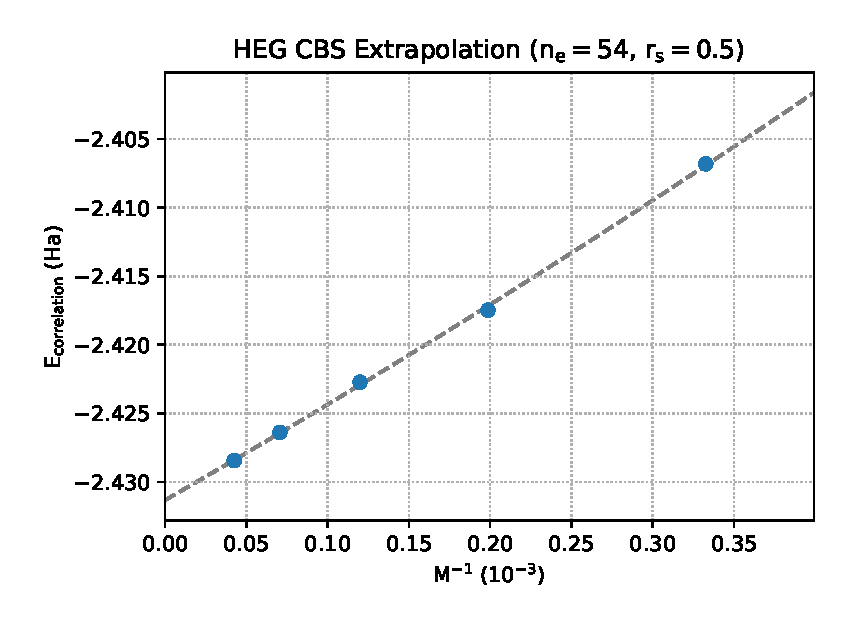
\includegraphics[width=\linewidth]{figs/cbs54e_05.eps}
  \end{center}
  \vspace{-0.2cm}
  \caption{Complete basis set extrapolation for HEG 54-electron supercell with $r_s=0.5$.
  The extrapolated correlation energy is $-2.4313(11)$~Ha.
  }
  \label{fig:cbs54e_05}
\end{figure}
\begin{table}
\caption{Summary of the HEG Total Correlation Energies~(Ha) with 54-Electron Supercells.
DMC~\cite{rios2006inhomogeneous} uses real space basis and backflow wave function.
FCIQMC~\cite{shepherd2012full} and its recent improvement FCIQMC-TC~\cite{luo2018combining} use up to 1850 orbitals.
SHCI uses up to 23506 orbitals, which give much shorter extrapolation distances than FCIQMC and thus more accurate results.
}
\label{tab:results54}
\begin{tabular}{| c || c || c | c | c | c |}
 \hline
 $r_s$ & SHCI & FCIQMC & FCIQMC-TC & BF-DMC \\
 \hline\hline
 0.5 & -2.4313(11) & -2.435(7) & -2.425(1) & -2.387(2) \\
 \hline
 % DMC~\cite{rios2006inhomogeneous}
%  \hline
%  54 & 0.5 & -2.4316(6) & - & -2.435(7) & -2.387(2) \\
%  \hline
%  54 & 1.0 & -2.114(2) & - & -2.124(3) &  -2.125(2) \\
 \hline
\end{tabular}
\end{table}

\section{Conclusions}
In this paper, we apply our fast semistochastic heat-bath configuration interaction algorithm (SHCI) to the homongenous electron gas (HEG) problem in the mid to high density region.
The basis set incompleteness error is a dominating error in this region, and the uncertainty of the result depends a lot on the uncertainty of the extrapolation, which in terms depends on the extrapolation distance.
By using SHCI with up to 39886 orbitals, we reduce the extrapolation distance significantly and achieves more accurate results than state-of-the-art methods.

\label{conclusions}

\section{Acknowledgements}
This work was supported by the AFOSR through grant FA9550-18-1-0095.
% A.A.H was supported by the NSF under the grant ACI-1534965 and by the University of Colorado.
% S.S. acknowledges the funding provided by the NSF through grant CHE-1800584.
%The computations were performed on the Bridges cluster at the Pittsburgh Supercomputing Center under NSF grant ACI-1445606,
%and on the Cooley and Theta clusters at Argonne National Laboratory.
%This work used the Extreme Science and Engineering Discovery Environment (XSEDE), which is supported by National Science Foundation grant number ACI-1548562. Specifically, it used the Bridges system, which is supported by NSF award number ACI-1445606, at the Pittsburgh Supercomputing Center (PSC).
Some computations were performed on the Bridges cluster at the Pittsburgh Supercomputing Center supported by NSF grant ACI-1445606, as part of the XSEDE program supported by NSF grant ACI-1548562.
We also acknowledge the support from Google Cloud Platform.
%and the Argonne Leadership Computing Facility (ALCF) at the Argonne National Laboratory.
% This research also used a Director’s Discretionary allocation at the Argonne Leadership Computing Facility, which is
% a DOE Office of Science User Facility supported under Contract DE-AC02-06CH11357.

%\appendix

\section{HEG Hamiltonian}
\label{app:heg}
We consider a system of $N_\uparrow$ spin-up electrons and $N_\downarrow$ spin-down electrons in a $d$-dimensional hypercube of side length $L$ with periodic boundary conditions in all directions and a uniform positive background such that the whole system is neutral.

The Hamiltonian of this system can be expressed in terms of the Yukawa potential $V\left( {\mathbf{r};\kappa } \right) = \frac{{{e^{ - \kappa r}}}}{r}$
\begin{align*}
\hat{H}=\sum_{i=1}^{N}-\frac{1}{2}\nabla_i^2+\frac{1}{2}\sum_{i\ne j}^{N} \frac{1}{L^d}\sum_{\mathbf{q}\ne 0}V(\mathbf{q})e^{i\mathbf{q}\cdot(\mathbf{r}_i-\mathbf{r}_j)}
\end{align*}
where 
$N= N_\uparrow + N_\downarrow$,
$\mathbf{q}=\frac{2\pi}{L}(n_1, n_2, \cdots, n_d)$, $n_i\in\Bbb{Z}$.
And $V(\mathbf{q})$ is the Fourier transform of the Yukawa potential at $\kappa\to 0$.
For $d=3$, $V(\mathbf{q})=\frac{4\pi}{q^2}$. \cite{giuliani2005quantum}

To convert the Hamiltonian into its second quantization form
$$\hat{H}=\sum_{PQ}f_{PQ}a_P^\dag a_Q+\frac{1}{2}\sum_{PQRS}g_{PQRS}a_P^\dag a_R^\dag a_Qa_S$$
we use the planewave basis set
$$\phi_P(x)=\frac{1}{\sqrt{L^d}}e^{-i\mathbf{k}_P\cdot\mathbf{r}}\sigma_P(m_s)$$
where $\sigma_P(m_s)$ is the spin eigenfunction and $\mathbf{k}_P=\frac{2\pi}{L}(n_{P_1}, n_{P_2},\cdots, n_{P_d})$, $n_{P_i}\in\Bbb{Z}$.

After simplification, we can get the coefficients of the second quantization terms
\begin{align*}
f_{PQ}= & \frac{\mathbf{k}_Q^2}{2}\delta_{\sigma_P\sigma_Q}\delta_{\mathbf{k}_P\mathbf{k}_Q}\\
g_{PQRS}= & \frac{1}{L^d}\delta_{\sigma_P\sigma_Q}\delta_{\sigma_R\sigma_S}V(\mathbf{k}_{PQ})\\
& (1-\delta_{\mathbf{k}_Q\mathbf{k}_P})\delta_{\mathbf{k}_Q+\mathbf{k}_S,\mathbf{k}_P+\mathbf{k}_R}
\end{align*}

Hence, the Hamiltonian matrix elements between a pair of Slater determinants are
\begin{align*}
\langle i|\hat{H}|i\rangle  = & \sum_{P}i_P\frac{\mathbf{k}_P^2}{2}-\frac{1}{2L^d}\sum_{P\ne R}i_Pi_R\delta_{\sigma_P\sigma_R}V(\mathbf{k}_{RP})\\
\langle i_1|\hat{H}|i_2\rangle  = &  \Gamma_I^{i_1}\Gamma_J^{i_1}\Gamma_K^{i_2}\Gamma_L^{i_2}\delta_{\mathbf{k}_K+\mathbf{k}_L,\mathbf{k}_I+\mathbf{k}_J}\frac{1}{L^d}\\
&  \lbrack\delta_{\sigma_I\sigma_K}\delta_{\sigma_J\sigma_L}V(\mathbf{k}_{IK})-\delta_{\sigma_I\sigma_L}\delta_{\sigma_J\sigma_K}V(\mathbf{k}_{IL})\rbrack
\end{align*}
where $i_P=1$ if and only if orbital $i$ is occupied, $\Gamma_P^i=\sum_{l=1}^{P-1}(-1)^{i_l}$. $|i_1\rangle$ has orbitals $I,J$ occupied while $|i_2\rangle$ has orbitals $K,L$ occupied, $I<J$, $K<L$, and all the other orbitals of $|i_1\rangle$ and $|i_2\rangle$ are the same.
\appendix

\section{HEG Hamiltonian}
\label{app:heg}
We consider a system of $N_\uparrow$ spin-up electrons and $N_\downarrow$ spin-down electrons in a $d$-dimensional hypercube of side length $L$ with periodic boundary conditions in all directions and a uniform positive background such that the whole system is neutral.

The Hamiltonian of this system can be expressed in terms of the Yukawa potential $V\left( {\mathbf{r};\kappa } \right) = \frac{{{e^{ - \kappa r}}}}{r}$
\begin{align*}
\hat{H}=\sum_{i=1}^{N}-\frac{1}{2}\nabla_i^2+\frac{1}{2}\sum_{i\ne j}^{N} \frac{1}{L^d}\sum_{\mathbf{q}\ne 0}V(\mathbf{q})e^{i\mathbf{q}\cdot(\mathbf{r}_i-\mathbf{r}_j)}
\end{align*}
where 
$N= N_\uparrow + N_\downarrow$,
$\mathbf{q}=\frac{2\pi}{L}(n_1, n_2, \cdots, n_d)$, $n_i\in\Bbb{Z}$.
And $V(\mathbf{q})$ is the Fourier transform of the Yukawa potential at $\kappa\to 0$.
For $d=3$, $V(\mathbf{q})=\frac{4\pi}{q^2}$. \cite{giuliani2005quantum}

To convert the Hamiltonian into its second quantization form
\beq
\hat{H}=\sum_{PQ}f_{PQ}a_P^\dag a_Q+\frac{1}{2}\sum_{PQRS}g_{PQRS}a_P^\dag a_Q^\dag a_Ra_S
\eeq
we use the planewave basis set
\beq
\phi_P(x)=\frac{1}{\sqrt{L^d}}e^{-i\mathbf{k}_P\cdot\mathbf{r}}\sigma_P(m_s)
\eeq
where $\sigma_P(m_s)$ is the spin eigenfunction and $\mathbf{k}_P=\frac{2\pi}{L}(n_{P_1}, n_{P_2},\cdots, n_{P_d})$, $n_{P_i}\in\Bbb{Z}$.

After simplification, we can get the coefficients of the second quantization terms
\begin{align*}
f_{PQ}= & \frac{\mathbf{k}_Q^2}{2}\delta_{\sigma_P\sigma_Q}\delta_{\mathbf{k}_P\mathbf{k}_Q}\\
g_{PQRS}= & \frac{1}{L^d}\delta_{\sigma_P\sigma_R}\delta_{\sigma_Q\sigma_S}V(\mathbf{k}_{PR})\\
& (1-\delta_{\mathbf{k}_R\mathbf{k}_P})\delta_{\mathbf{k}_R+\mathbf{k}_S,\mathbf{k}_P+\mathbf{k}_Q}
\end{align*}

Hence, the Hamiltonian matrix elements between a pair of Slater determinants are
\begin{align*}
\langle i|\hat{H}|i\rangle  = & \sum_{P}i_P\frac{\mathbf{k}_P^2}{2}-\frac{1}{2L^d}\sum_{P\ne Q}i_Pi_Q\delta_{\sigma_P\sigma_Q}V(\mathbf{k}_{QP})\\
\langle i_1|\hat{H}|i_2\rangle  = &  \Gamma_I^{i_1}\Gamma_J^{i_1}\Gamma_K^{i_2}\Gamma_L^{i_2}\delta_{\mathbf{k}_K+\mathbf{k}_L,\mathbf{k}_I+\mathbf{k}_J}\frac{1}{L^d}\\
&  \lbrack\delta_{\sigma_I\sigma_K}\delta_{\sigma_J\sigma_L}V(\mathbf{k}_{IK})-\delta_{\sigma_I\sigma_L}\delta_{\sigma_J\sigma_K}V(\mathbf{k}_{IL})\rbrack
\end{align*}
where $i_P=1$ if and only if orbital $P$ is occupied, $\Gamma_P^i=\sum_{l=1}^{P-1}(-1)^{i_l}$. $|i_1\rangle$ has orbitals $I,J$ occupied while $|i_2\rangle$ has orbitals $K,L$ occupied, $I<J$, $K<L$, and all the other orbitals of $|i_1\rangle$ and $|i_2\rangle$ are the same.

%\bibliography{main}
%\bibliography{all}
\bibliography{alavi,main,hci,ceperley,needs,qmc,toulouse,umrigar}

\end{document}
%
% ****** End of file apssamp.tex ******
